\documentclass[12pt]{report}
\usepackage[utf8]{inputenc}
\usepackage{hyperref}
\usepackage{float}
\hypersetup{
    colorlinks,
    citecolor=black,
    filecolor=black,
    linkcolor=black,
    urlcolor=black
}
\usepackage{graphicx}
\usepackage{subcaption}
\usepackage[table,xcdraw]{xcolor}
\usepackage{colortbl}
\usepackage{multirow}
\usepackage{makecell}
%\usepackage[export]{adjustbox}
% redefine the Chapter title style (from Chapter 1 ... to 1. ...)
\makeatletter
\def\@makechapterhead#1{%
  \vspace*{0\p@}%
  {\parindent \z@ \raggedright \normalfont
    \ifnum \c@secnumdepth >\m@ne
      %\if@mainmatter
        %\huge\bfseries \@chapapp\space \thechapter
        \Huge\bfseries \thechapter.\space%
        %\par\nobreak
        %\vskip 20\p@
      %\fi
    \fi
    \interlinepenalty\@M
    \Huge \bfseries #1\par\nobreak
    \vskip 40\p@
  }}
\makeatother

% alias for 2 \newline command
\newcommand{\nnl}{%
    \newline
    \newline
}

% alias for \newline \noindent command
\newcommand{\nl}{%
    \newline
    \noindent
}

\title{\textbf{Report Machine Learning \& Pattern Recognition Project}}
\author{\textit{s314913 Gabriele Lorenzo}}
\date{July 2024}

\begin{document}

\maketitle

\begin{abstract}
    This report is the result of the project for the course of Machine Learning and Pattern Recognition. The project is about fingerprint spoofing detection. The dataset consists of labeled samples corresponding to the genuine (True, label 1) class and the fake (False, label 0) class. We will analyze the features of the dataset, perform dimensionality reduction, train and validate the classifiers on the training dataset, and finally test the classifiers on the testing dataset. We will use different classifiers: Gaussian Classifiers, Logistic Regression, Support Vector Machine, and Gaussian Mixture Model. We will evaluate the classifiers based on the error rate and the Detection Cost Function (DCF).
\end{abstract}

\tableofcontents

\chapter{Overview}
The main project task is to create a classifier that allow us to reliably do what is called fingerprint spoofing detection.
We can view this task as a \textbf{binary classification} problem where we have to distinguish genuine and counterfeit fingerprints.
\nnl
The dataset consists of labeled samples corresponding to the genuine (True, label 1) class and the fake (False, label 0) class.
Samples are computed by a feature extractor that summarizes high-level characteristics of a fingerprint image.
Both training and testing dataset are 6-dimensional, with the training data having 6000 samples and the testing data having also 6000 samples.

\chapter{Feature Analysis}
\section{Preliminary Analysis}
The first step is to analyze the features of the dataset.
\nnl
We will plot the histograms of the features for the genuine and fake classes.

\begin{figure}[H]
    \centering
    \begin{subfigure}[t]{0.49\textwidth}
        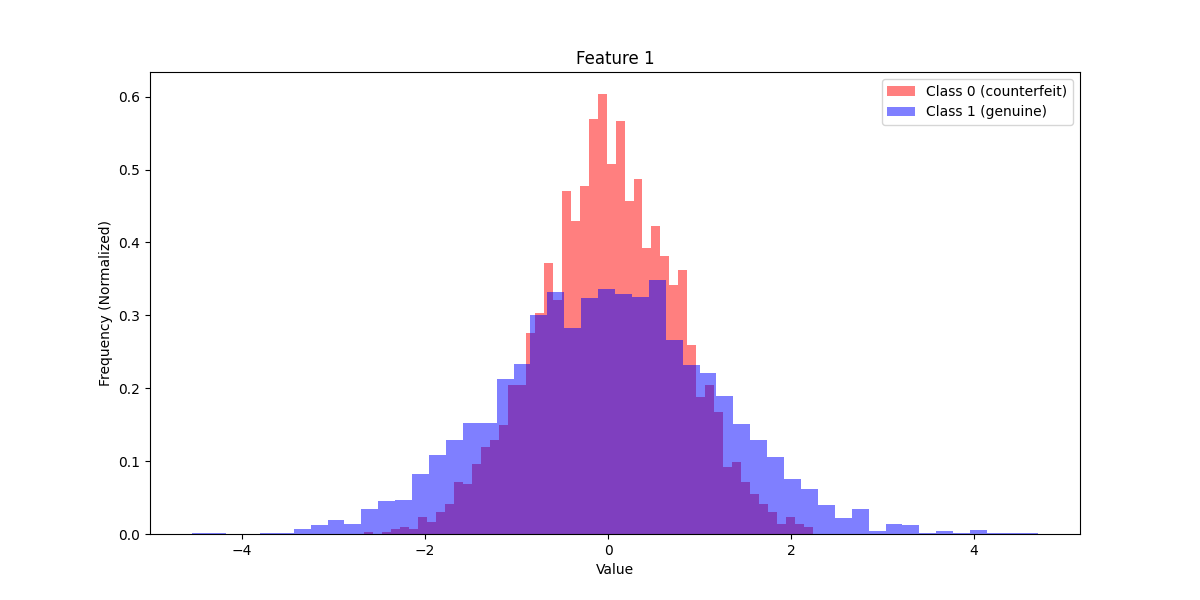
\includegraphics[width=\textwidth]{./plot/features/feature_1.png}
    \end{subfigure}
    \hfill
    \begin{subfigure}[t]{0.49\textwidth}
        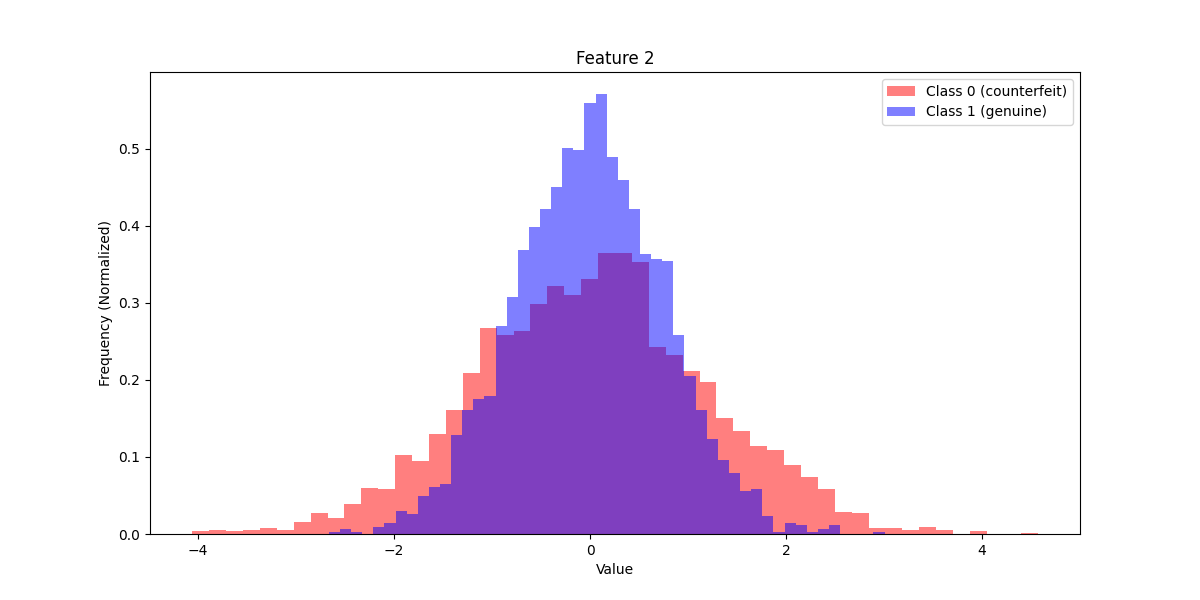
\includegraphics[width=\textwidth]{./plot/features/feature_2.png}
    \end{subfigure}
    %%%%%%%%%%%%%%%%%%%%%%%%%%%%%%%%%%%%second row
    \begin{subfigure}[t]{0.49\textwidth}
        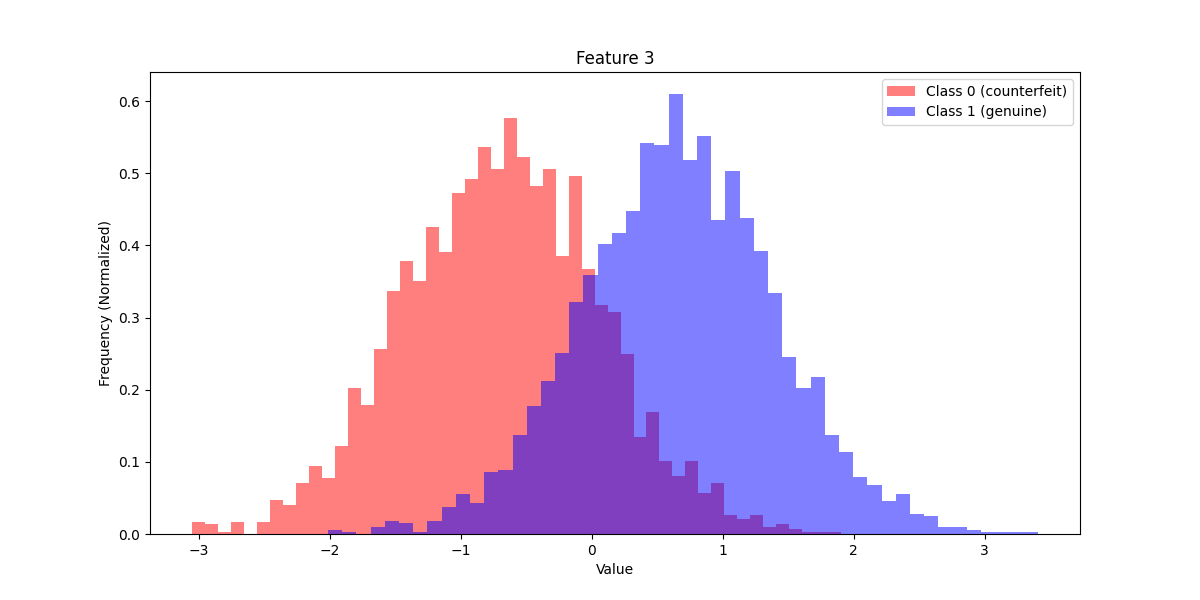
\includegraphics[width=\textwidth]{./plot/features/feature_3.png}
    \end{subfigure}
    \hfill
    \begin{subfigure}[t]{0.49\textwidth}
        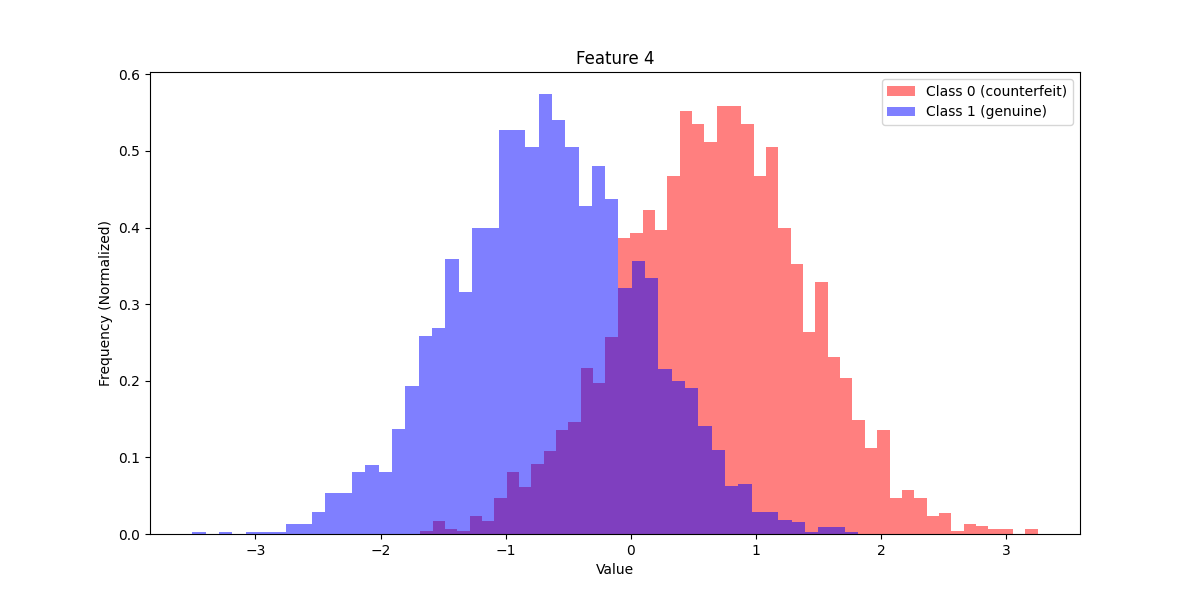
\includegraphics[width=\textwidth]{./plot/features/feature_4.png}
    \end{subfigure}
    %%%%%%%%%%%%%%%%%%%%%%%%%%%%%%%%%%%%third row
    \begin{subfigure}[t]{0.49\textwidth}
        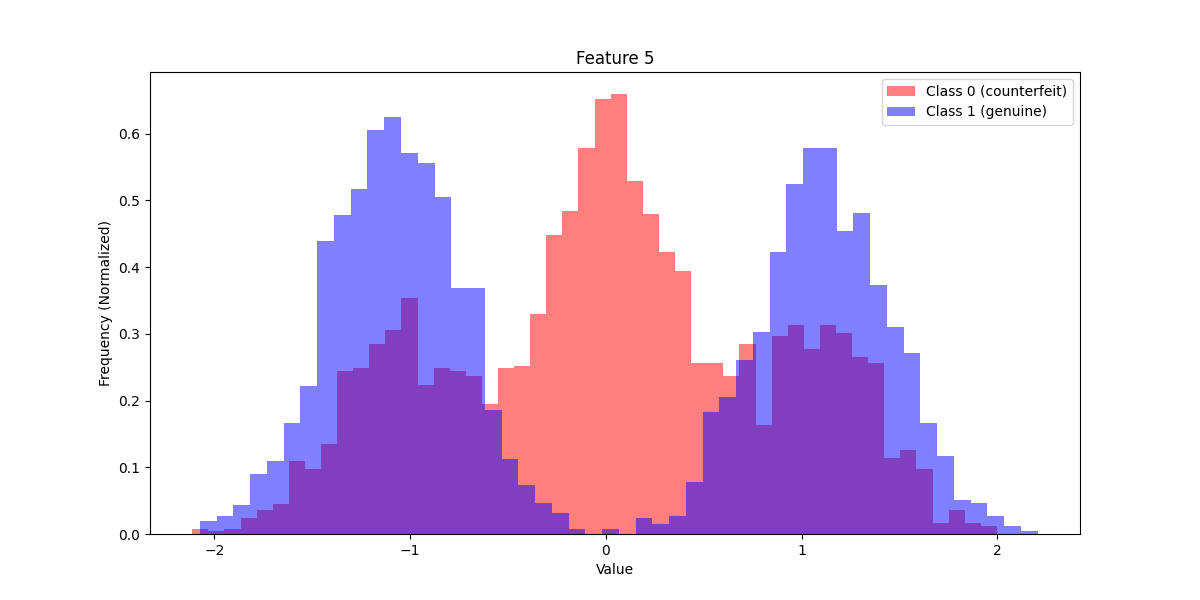
\includegraphics[width=\textwidth]{./plot/features/feature_5.png}
    \end{subfigure}
    \hfill
    \begin{subfigure}[t]{0.49\textwidth}
        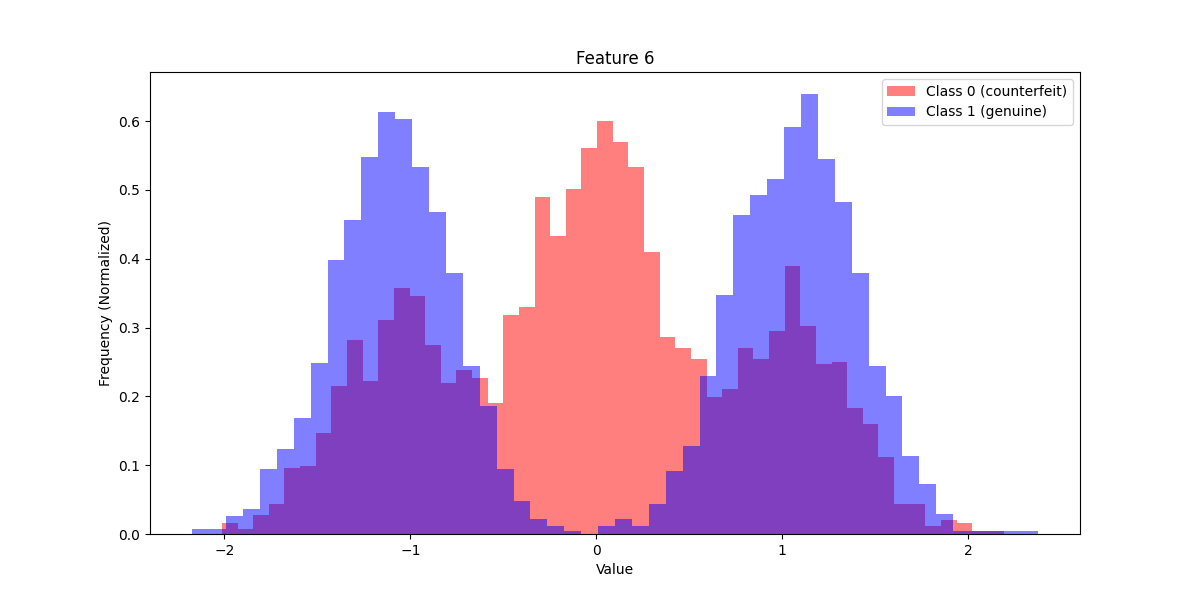
\includegraphics[width=\textwidth]{./plot/features/feature_6.png}
    \end{subfigure}
    \caption{Histograms of the features for the genuine and fake classes.}
    \label{fig:histograms}
\end{figure}
\noindent
As we can see the classes for features 1 and 2 have a similar mean, while their variance shows some differences: class 1 has higher variance than class 0 for feature 1 and lower variance than class 0 for feature 2. Both of the features are approximately gaussian distributed and the two classes overlap quite heavily on the middle part of the distribution. Since we can observe one main peak in our distributions (only one mode) we expect gaussian models to perform poorly.
\nnl
We observe that also features 3 and 4 are gaussian distributed and posses a similar variance, while their mean is different. The two classes overlap only in a portion of the distribution (since the means are quite different the overlap is only on the respective sides of the distributions). Here we can see two modes and gaussian models should clearly identify the two classes when using these features.
\nnl
Feature 5 and 6 are more complex. We observe three modes and the two features are not gaussian distributed. For both features class 1 can be modeled by two distinct gaussians, while class 0 can be modeled by a three gaussians (we can hence see two clusters for class 1 and three clusters for class 0). The two distributions overlap in the intervals corresponding to the two modes of class 1.
We expect gaussian mixture models to perform better than simple gaussian models for these features.
\nnl
We can also plot the pairwise plot of the features for the genuine and fake classes.

\begin{figure}[H]
    \centering
    \begin{subfigure}[t]{0.33\textwidth}
        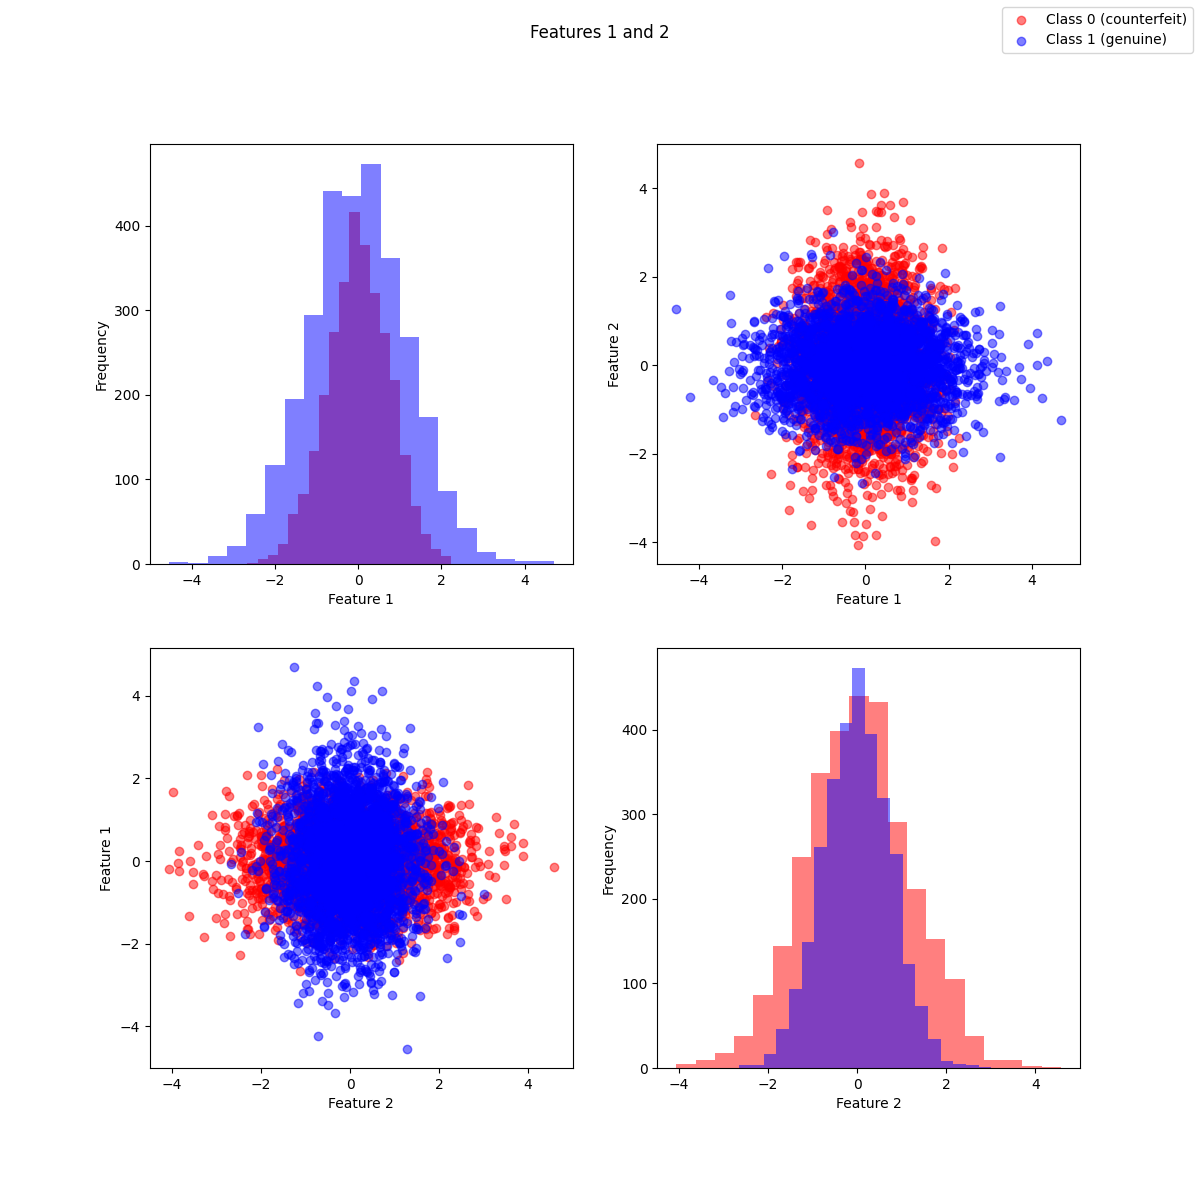
\includegraphics[width=\textwidth]{./plot/features/features_1_2.png}
    \end{subfigure}
    %%%%%%%%%%%%%%%%%%%%%%%%%%%%%%%%%%%%second row
    \begin{subfigure}[t]{0.33\textwidth}
        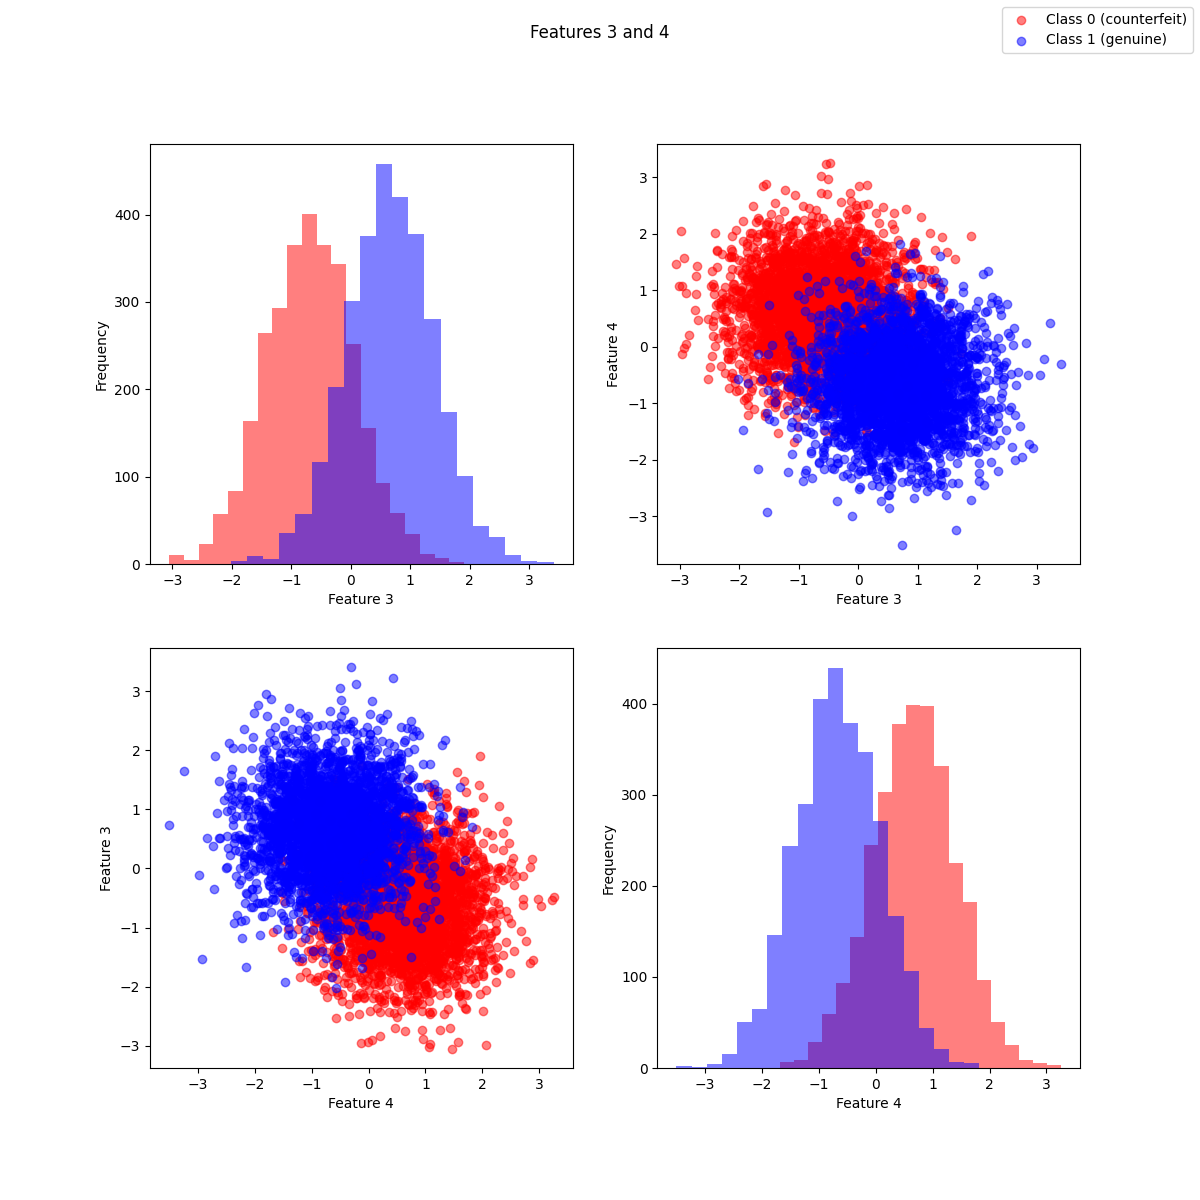
\includegraphics[width=\textwidth]{./plot/features/features_3_4.png}
    \end{subfigure}
    %%%%%%%%%%%%%%%%%%%%%%%%%%%%%%%%%%%%second row
    \begin{subfigure}[t]{0.32\textwidth}
        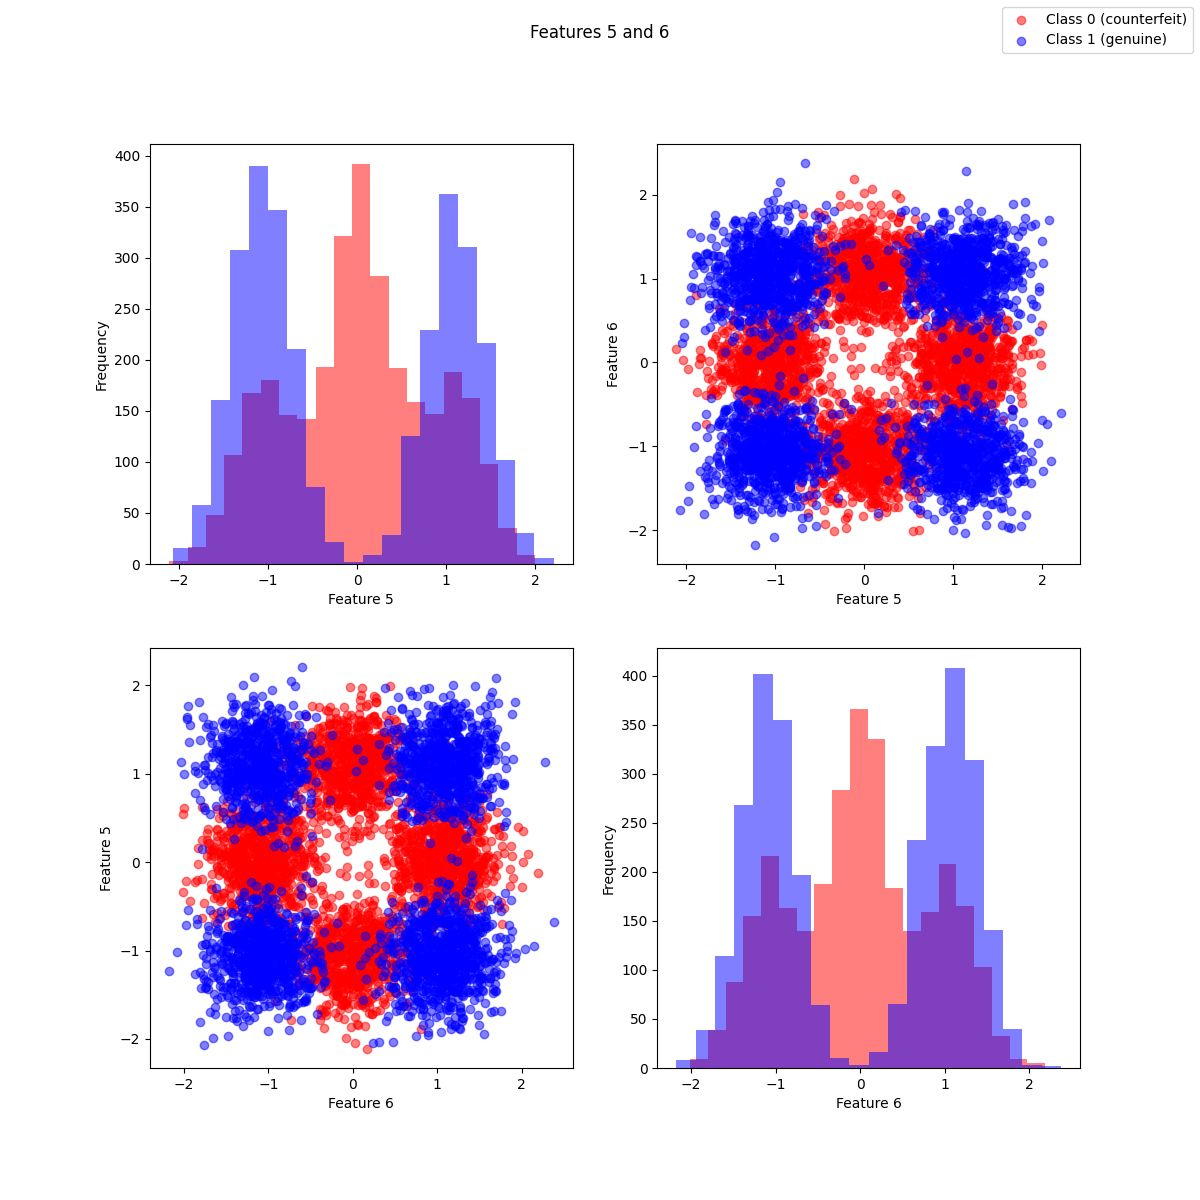
\includegraphics[width=\textwidth]{./plot/features/features_5_6.png}
    \end{subfigure}
    \caption{Pairwise plot of the features for the genuine and fake classes.}
    \label{fig:pairwise_plot}
\end{figure}
\noindent
The analysis previous analysis is confirmed by the pairwise plot of the features. We can see a string overlap for both classes in features 1 and 2, while we can see a separation in features 3 and 4. Features 5 and 6 show a more complex structure with more clusters for each class.
\nnl
Finally we can plot a pairwise plot of every feature with every other feature.
\begin{figure}[H]
    \centering
    \begin{subfigure}[t]{1\textwidth}
        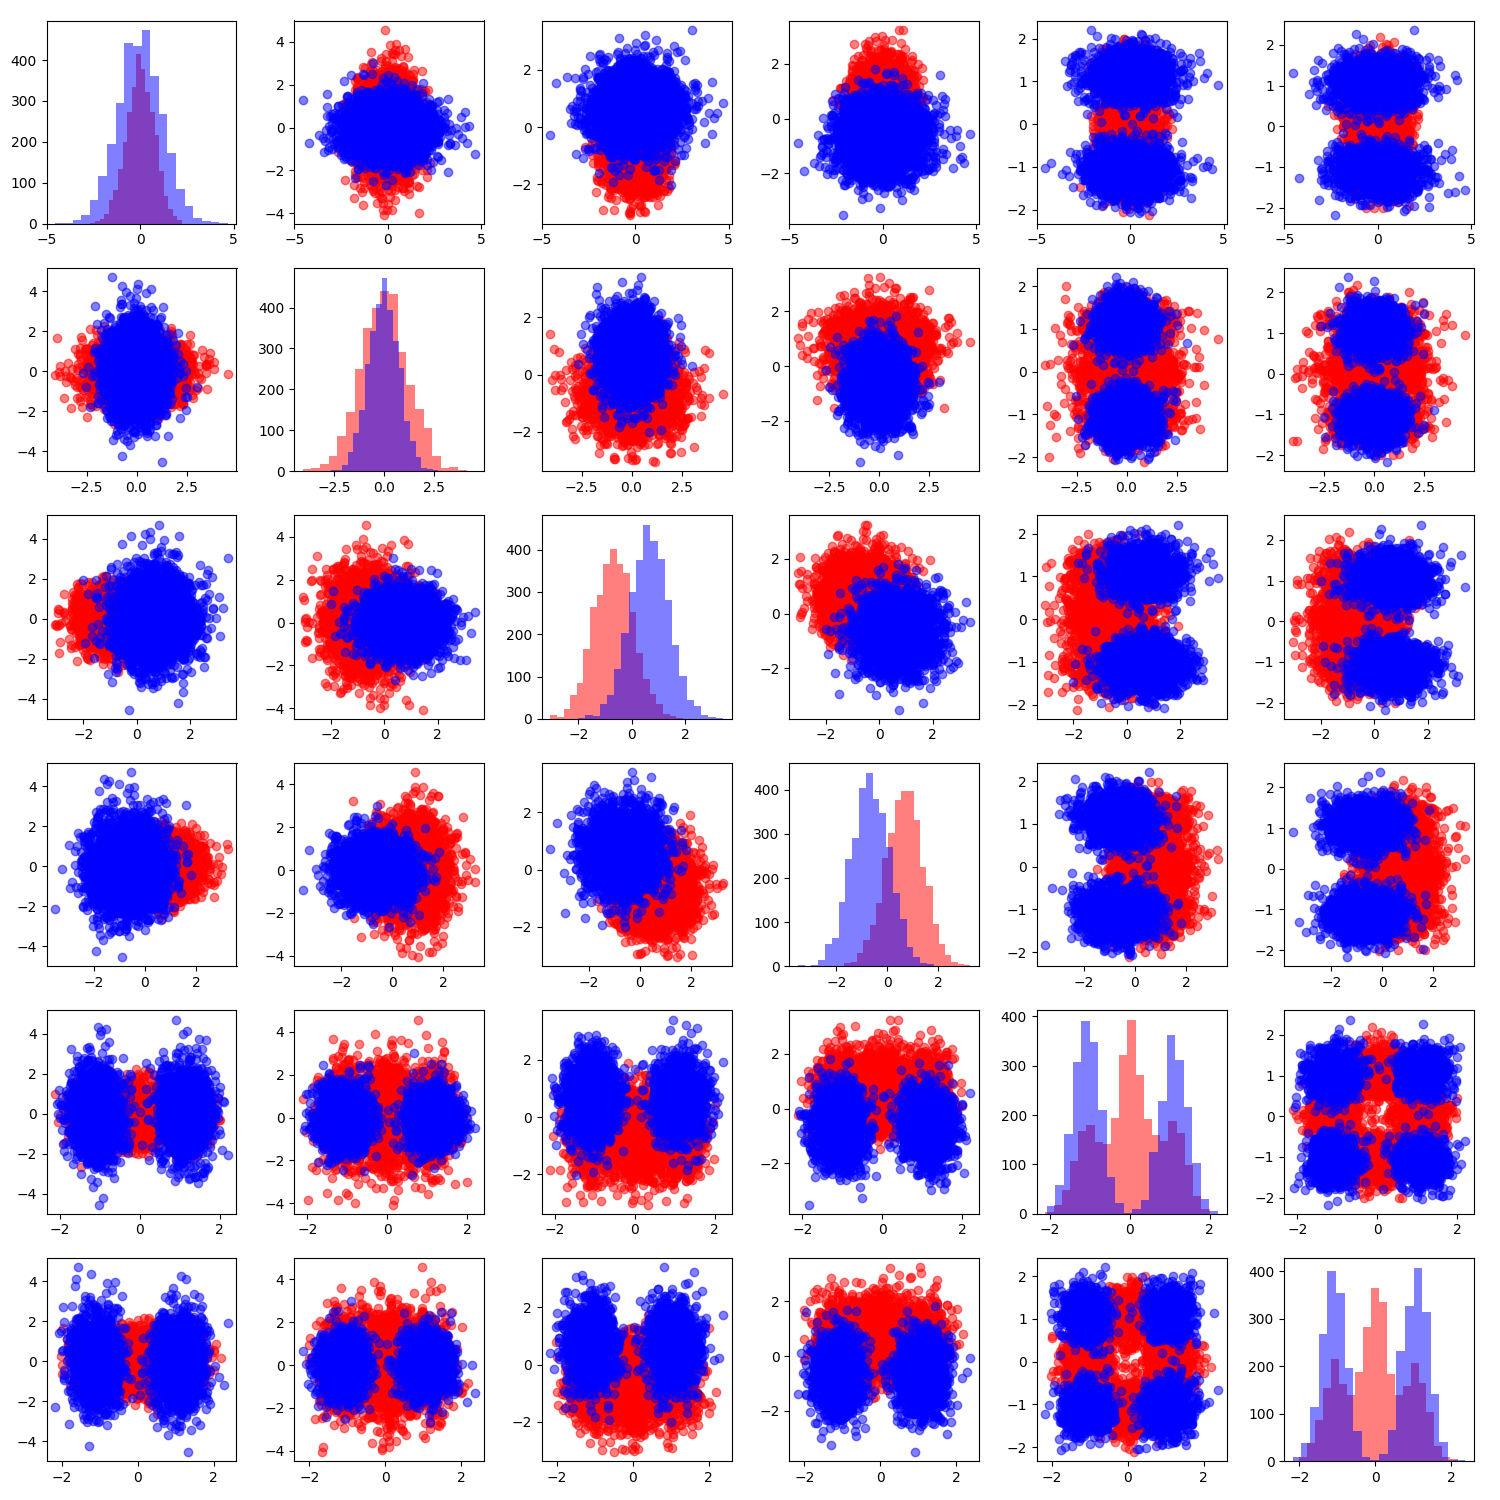
\includegraphics[width=\textwidth]{./plot/features/features_all.png}
    \end{subfigure}
    \caption{Pairwise plot of every feature with every other feature.}
    \label{fig:pairwise_plot_all}
\end{figure}
\noindent
From this preliminary analysis we can see that the features are not perfectly linearly separable and that we might to use more complex models to classify the samples.

\section{Gaussian Feature Analysis}
\label{sec:gauss_analysis}
We proceed to refine our analysis by fitting a gaussian model to the data.
\begin{figure}[H]
    \centering
    \begin{subfigure}[t]{1\textwidth}
        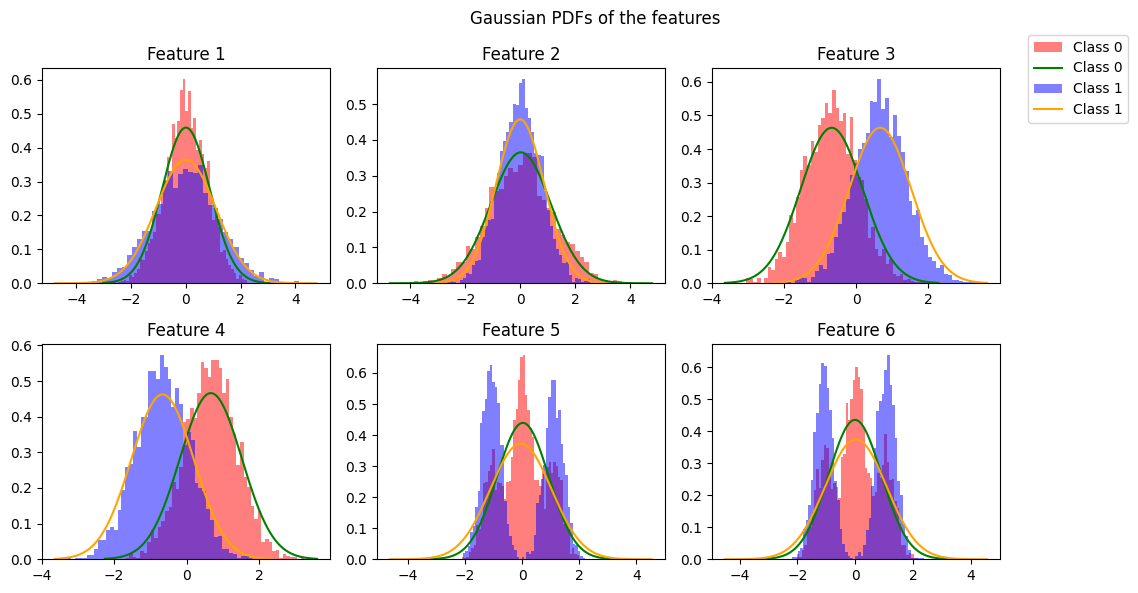
\includegraphics[width=\textwidth]{./plot/gauss_analysis/gaussian_analysis.png}
    \end{subfigure}
    \caption{Gaussian model fitted on each feature.}
    \label{fig:gauss_analysis}
\end{figure}
\noindent
As previously stated, there are discrepancies between the distributions of the two classes for each feature.
\nl
We can see that features 3 and 4 are the most promising for a gaussian model, while features 5 and 6 are the least promising. We will probably need to use a gaussian mixture model or other more complex non linear models to classify the samples.

\chapter{Dimensionality Reduction}
To gain more insight into the data we can perform dimensionality reduction using PCA and LDA.
\nnl
We will first start by using PCA and project our data on the 6 PCA directions, starting from the direction with the highest variance.
In the following we will refer to PCA components as the projection of data on the PCA directions.
\begin{figure}[H]
    \centering
    \begin{subfigure}[t]{1\textwidth}
        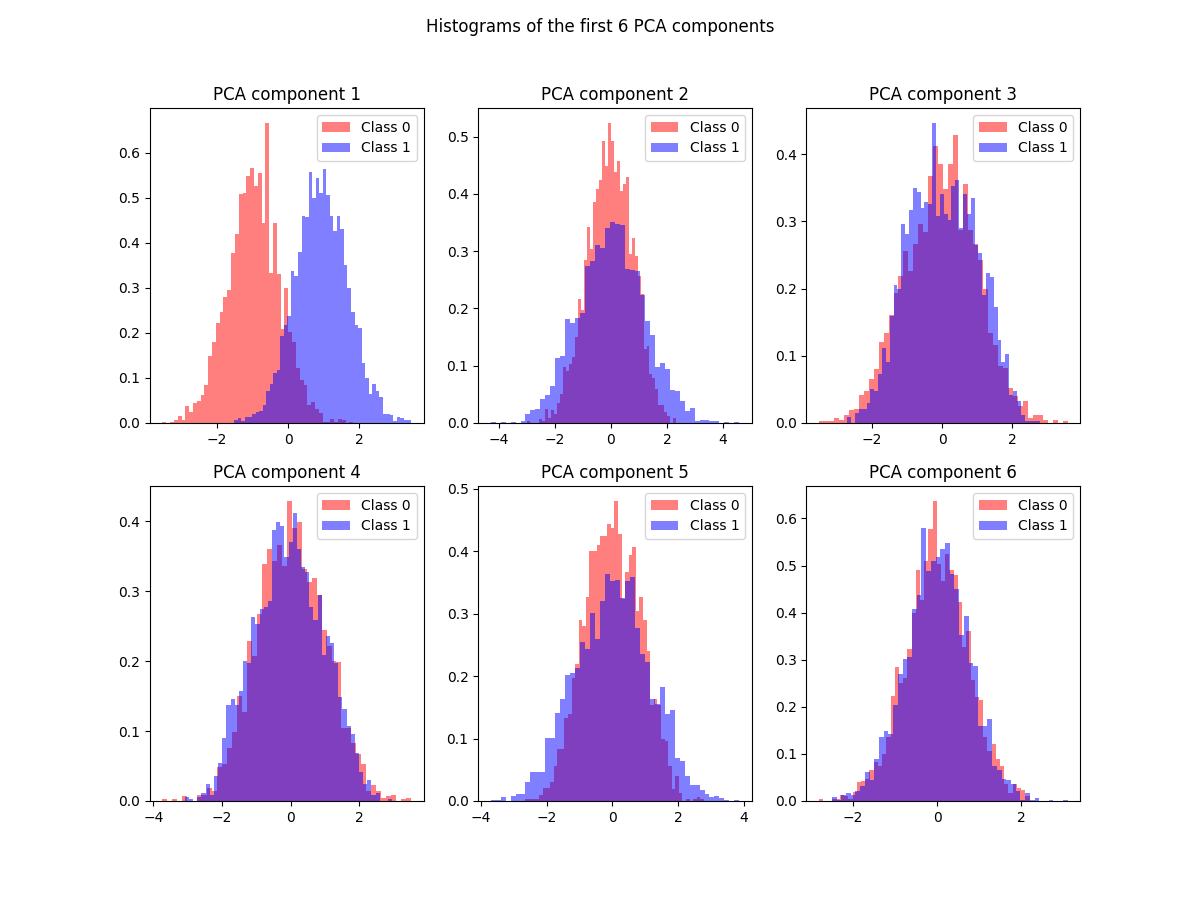
\includegraphics[width=\textwidth]{./plot/dim_red/PCA.png}
    \end{subfigure}
    \caption{PCA projection of the data.}
    \label{fig:PCA}
\end{figure}
\noindent
As we can see, the first PCA component is able to separate the two classes quite well, while the rest of the components do worst at separating the two classes.
\nnl
Now we can use LDA to project the data on the first LDA direction.
\begin{figure}[H]
    \centering
    \begin{subfigure}[t]{0.6\textwidth}
        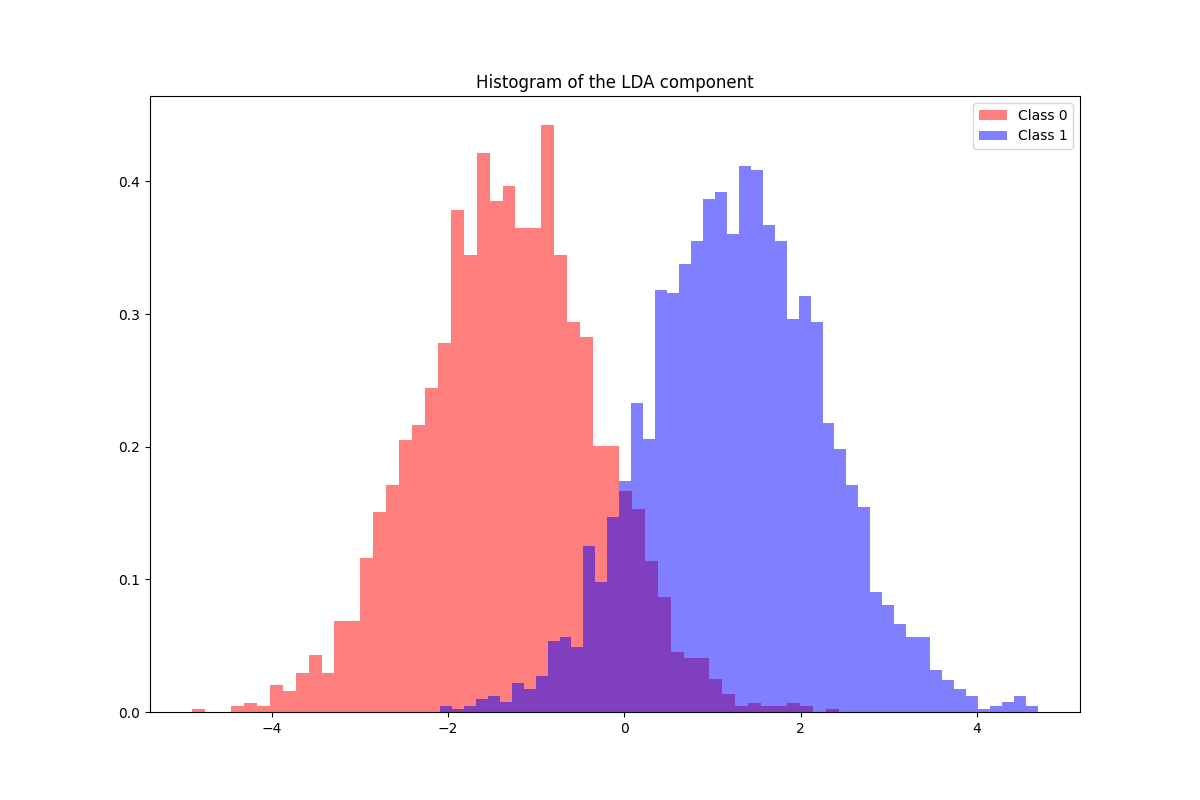
\includegraphics[width=\textwidth]{./plot/dim_red/LDA.png}
    \end{subfigure}
    \caption{Histogram of LDA projection of data.}
    \label{fig:LDA}
\end{figure}
\noindent
After applying LDA the classes overlap only on a partial portion of the distribution. This is a good result since we want to have a clear separation between the two classes.
\nl
Compared to \autoref{fig:histograms} we can see that the LDA projection is able to separate the two classes better than the original features.
\nnl
In the following part, we will attempt out first classification, using LDA as a classifier.
\nl
We first divide our training dataset in a training and validation part. From now on, if not stated otherwise, we will always do a single split with a training/validation ratio of 2:1.
\nnl
Here is the histogram plot of the validation data and the threshold given by the average of the projected class means:
\begin{figure}[H]
    \centering
    \begin{subfigure}[t]{0.7\textwidth}
        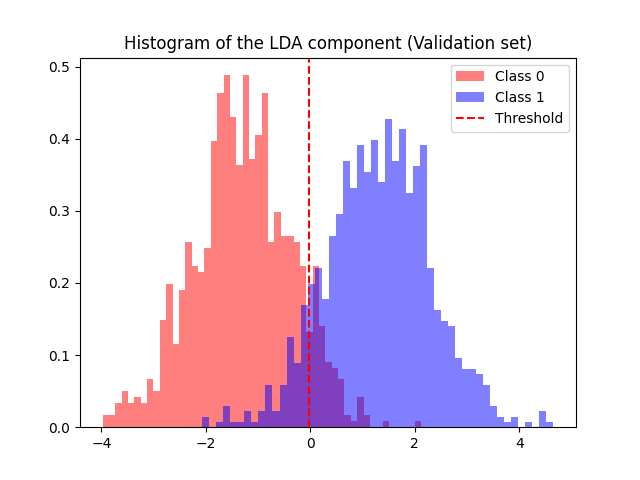
\includegraphics[width=\textwidth]{./plot/dim_red/LDA_threshold_base.png}
    \end{subfigure}
    \caption{Histogram of LDA projection of data and simple threshold.}
    \label{fig:LDA_threshold_base}
\end{figure}
\noindent
Here instead we use a optimized threshold, calculated by iterating over all the possible values ad finding the best, that minimizes the error rate:
\begin{figure}[H]
    \centering
    \begin{subfigure}[t]{0.7\textwidth}
        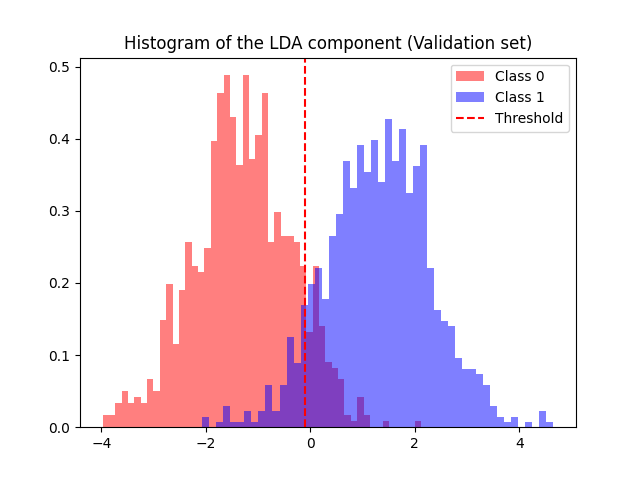
\includegraphics[width=\textwidth]{./plot/dim_red/LDA_threshold_opt.png}
    \end{subfigure}
    \caption{Histogram of LDA projection of data and optimized threshold.}
    \label{fig:LDA_threshold_opt}
\end{figure}
\noindent
\nl
As we can see the two thresholds are not too far apart. We can expect the errors rates to be similar for both thresholds.
\nl
The error rates are presented in this table:
\begin{table}[H]
    \centering
    \begin{tabular}{|c|c|c|}
        \rowcolor{blue!10}
        \hline
                            & \textbf{Simple Threshold} & \textbf{Optimized Threshold} \\
        \hline
        \textbf{Error Rate} & 9.10\%                    & 9.10\%                       \\
        \hline
    \end{tabular}
    \caption{Error rates for LDA classifier.}
    \label{tab:LDA_error}
\end{table}
\noindent
We can improve the classification by applying preprocessing to the data by means of PCA. As before we are going to try using first the simple threshold and then the optimized threshold for the classification.
\nl
The final results are presented in this table:
\begin{table}[H]
    \centering
    \begin{tabular}{|c|c|c|}
        \hline
        \rowcolor{blue!10}
        \textbf{PCA m components} & \textbf{Simple Threshold} & \textbf{Optimized Threshold}      \\
        \hline
        \textbf{m=1}              & 90.65\%                   & 55\%                              \\
        \hline
        \textbf{m=2}              & \textcolor{cyan}{9.25\%}  & \textcolor{cyan}{\textbf{8.95\%}} \\
        \hline
        \textbf{m=3}              & \textcolor{cyan}{9.25\%}  & 9.15\%                            \\
        \hline
        \textbf{m=4}              & \textcolor{cyan}{9.25\%}  & 9.15\%                            \\
        \hline
        \textbf{m=5}              & 9.30\%                    & 9.05\%                            \\
        \hline
        \textbf{m=6}              & 9.30\%                    & 9.10\%                            \\
        \hline
    \end{tabular}
    \caption{Error rates for LDA classifier with PCA preprocessing.}
    \label{tab:LDA_PCA_error}
\end{table}
\noindent
The best results in terms of error rate are obtained by using 2 PCA components and the optimized threshold, giving a lower error rate than the LDA classifier without PCA preprocessing.

\chapter{Training \& Validation}

\section{Introduction}
The main goal of this part is to train and validate the classifiers on the training dataset.
\nl
The classifiers we are going to use are:
\begin{itemize}
    \item Gaussian Classifiers
          \begin{itemize}
              \item Multivariate Gaussian (MVG)
              \item MVG with Naive Bayes assumption (Naive MVG)
              \item MVG with diagonal covariance matrix (Tied MVG)
          \end{itemize}
    \item Logistic Regression (LR)
    \item Support Vector Machine (SVM)
    \item Gaussian Mixture Model (GMM)
\end{itemize}
\noindent
As previously stated, we will use a single split of the training dataset in a training and validation part, with a ratio of 2:1.
\nl
In the beginning we will validate the classifiers based on the error rates they produce. We will then use a more complex metric, the Detection Cost Function (DCF), to evaluate the classifiers.
\nl
The DCF is a metric that takes into account the cost of false positives and false negatives.
\nl
We define the un-normalized DCF as:
\begin{equation}
    DCF_{u} = \pi_{T}  C_{fn}  P_{fn} + (1-\pi_{T})  C_{fp}  P_{fp}
\end{equation}
Where $\pi_{T}$ is the prior probability of the target class (1), $C_{fn}$ is the cost of a false negative, $P_{fn}$ is the false negative rate ($P_{fn} = \frac{TN}{FN + TP}$), $C_{fp}$ is the cost of a false positive, and $P_{fp}$ is the false positive rate ($P_{fp} = \frac{FP}{FP + TN}$).
\nl
In particular we notice that the parameter $\pi_{T}$, $C_{fn}$, and $C_{fp}$ depend only on the application we are considering. We can summarize these parameters by computing what is called the effective prior:
\begin{equation}
    \tilde{\pi} = \frac{\pi_{T} C_{fn}}{\pi_{T} C_{fn} + (1-\pi_{T}) C_{fp}}
\end{equation}
\nl
We can thus rewrite the un-normalized DCF as:
\begin{equation}
    DCF_{u} = \tilde{\pi} P_{fn} + (1-\tilde{\pi}) P_{fp}
\end{equation}
\nl
To have a more meaningful metric we can normalize the DCF by the DCF of a dummy classifier:
\begin{equation}
    DCF = \frac{DCF_{u}(\pi_T,C_{fn},C_{fp})}{min(\pi_{T}  C_{fn},(1-\pi_{T})  C_{fp})}
\end{equation}
The normalized DCF is invariant to scaling, so it has the same value whether we use or no we use the effective prior.
\nnl
Now that we have clearly defined the framework we are going to use, we can proceed with the training and validation of the classifiers.

\section{Multivariate Gaussian Classifier}
Here are the results of the Gaussian classifiers and LDA classifier in terms of error rate:

\begin{table}[H]
    \centering
    \begin{tabular}{|c|c|}
        \hline
        \rowcolor{blue!10}
        \textbf{Classifier} & \textbf{Error Rate}               \\
        \hline
        MVG                 & \textcolor{cyan}{\textbf{7.00\%}} \\
        \hline
        Naive MVG           & 7.20\%                            \\
        \hline
        Tied MVG            & 9.30\%                            \\
        \hline
        LDA                 & 9.10\%                            \\
        \hline
    \end{tabular}
    \caption{Error rates for MVG classifiers and LDA classifier.}
    \label{tab:MVG_error}
\end{table}
\noindent
The MVG classifier performs the best in terms of error rate, followed by the Naive MVG classifier.
Both the LDA and Tied MVG classifiers have a higher error rate than the other models.
This could suggest that the features are somewhat independent.
\nnl
To confirm this hypothesis we can compute the correlation matrix of the features:
\begin{figure}[H]
    \centering
    \begin{subfigure}[t]{0.8\textwidth}
        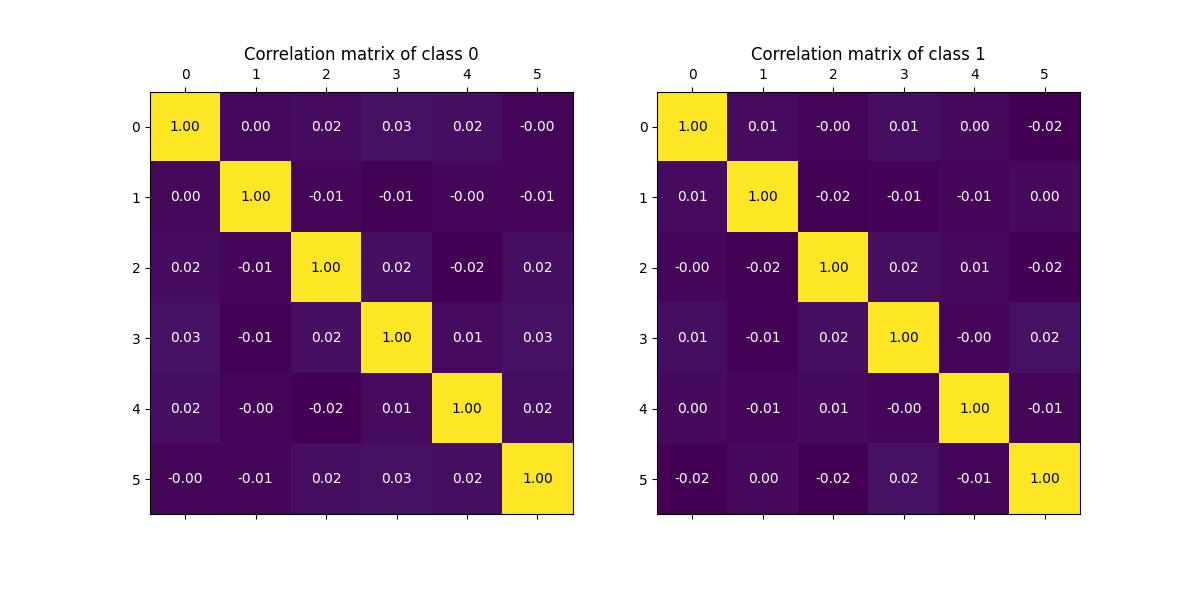
\includegraphics[width=\textwidth]{./plot/MVG/correlation_matrix.png}
    \end{subfigure}
    \caption{Correlation matrix of the features.}
    \label{fig:correlation_matrix}
\end{figure}
\noindent
As we can see the features are not correlated: the values of covariance among the different features are close to 0, confirming our hypothesis. We can thus see why the Naive MVG classifier performs better, since this classifier assumes that the features are independent.
\nnl
As discussed in \autoref{sec:gauss_analysis}, features 3 and 4 are the most promising for a gaussian model, while the others will presumably need a more complex model to classify the samples.
\nnl
We will now try to classify the samples using a subset of features.
\nl
We will start by using the first 4 features:
\begin{table}[H]
    \centering
    \begin{tabular}{|c|c|}
        \hline
        \rowcolor{blue!10}
        \textbf{Classifier} & \textbf{Error Rate}               \\
        \hline
        MVG                 & 7.95\%                            \\
        \hline
        Naive MVG           & \textcolor{cyan}{\textbf{7.65\%}} \\
        \hline
        Tied MVG            & 9.50\%                            \\
        \hline
        LDA                 & 9.15\%                            \\
        \hline
    \end{tabular}
    \caption{Error rates for MVG classifiers and LDA classifier using the first 4 features.}
    \label{tab:MVG_error_4}
\end{table}
\noindent
We observe that the performances are roughly the same (but slightly worse) than using all the features. This indicates that features 5 and 6 are not degrading the performances of the classifiers, but at the same time they offer few relevant information for the classification.
\nl
We'll proceed by classifying the samples using features 1 and 2 and then features 3 and 4 jointly.

\begin{table}[H]
    \centering
    \begin{tabular}{|c|c|}
        \hline
        \rowcolor{blue!10}
        \textbf{Classifier} & \textbf{Error Rate}                \\
        \hline
        MVG                 & 36.50\%                            \\
        \hline
        Naive MVG           & \textcolor{cyan}{\textbf{36.30\%}} \\
        \hline
        Tied MVG            & 49.45\%                            \\
        \hline
        LDA                 & 44.45\%                            \\
        \hline
    \end{tabular}
    \caption{Error rates for MVG classifiers and LDA classifier using features 1 and 2.}
    \label{tab:MVG_error_1_2}
\end{table}

\begin{table}[H]
    \centering
    \begin{tabular}{|c|c|}
        \hline
        \rowcolor{blue!10}
        \textbf{Classifier} & \textbf{Error Rate}                 \\
        \hline
        MVG                 & 9.45\%                              \\
        \hline
        Naive MVG           & 9.40\%                              \\
        \hline
        Tied MVG            & 9.45\%                              \\
        \hline
        LDA                 & \textcolor{cyan}{\textbf{9.10\%}}\% \\
        \hline
    \end{tabular}
    \caption{Error rates for MVG classifiers and LDA classifier using features 3 and 4.}
    \label{tab:MVG_error_3_4}
\end{table}
\noindent
These results confirm our previous analysis. Features 1 and 2 are not able to separate the two classes, while features 3 and 4 are able to do so in a more reliable way.
\nl
In particular, we can see that using features 1 and 2 the MVG and Naive MVG classifiers have the lowest error rate (for the naive case this can be explained by the low correlation between features).
\nl
The Tied MVG model performs the worst as expected. This is due to the fact that this model assumes that the covariance matrix is the same for both classes, but as discussed in \autoref{sec:gauss_analysis} the two classes have different variance for features 1 and 2.
\nl
A different outcome is observed for features 3 and 4: they have similar variance but different mean. Moreover these features have a weak correlation. All these factors can explain the good performances of the MVG classifiers wrt only using features 1 and 2.
\nnl
As a final step we will try to classify the samples using PCA as a preprocessing step.

\begin{table}[H]
    \centering
    \begin{tabular}{|c|c|c|c|c|c|}
        \hline
        \rowcolor{blue!10}
        \textbf{PCA m components} & \textbf{MVG}                      & \textbf{Naive MVG} & \textbf{Tied MVG} & \textbf{LDA} \\
        \hline
        \textbf{m=1}              & 9.25\%                            & 9.25\%             & 9.35\%            & 55.00\%      \\
        \hline
        \textbf{m=2}              & 8.80\%                            & 8.85\%             & 9.25\%            & 8.95\%       \\
        \hline
        \textbf{m=3}              & 8.80\%                            & 9.00\%             & 9.25\%            & 9.15\%       \\
        \hline
        \textbf{m=4}              & 8.05\%                            & 8.85\%             & 9.25\%            & 9.15\%       \\
        \hline
        \textbf{m=5}              & 7.10\%                            & 8.75\%             & 9.30\%            & 9.05\%       \\
        \hline
        \textbf{m=6}              & \textcolor{cyan}{\textbf{7.00\%}} & 8.90\%             & 9.30\%            & 9.10\%       \\
        \hline
    \end{tabular}
    \caption{Error rates for MVG classifiers and LDA classifier with PCA preprocessing.}
    \label{tab:MVG_PCA_error}
\end{table}
\noindent
PCA doesn't seem to be effective with this dataset. The best results are obtained by using 6 PCA components, but the error rate is the same than using the original features.
\nnl
After this preliminary analysis we can say that the best model is the MVG classifier (without preprocessing of data) with an error rate of 7.00\%.

\subsection*{Detection Cost Function analysis}
As discussed before, error rate can sometimes be misleading. We will now use a more robust metric, the DCF, to evaluate the MVG classifiers.
\nl
We will start by using 5 different applications with different values of $\pi_{T}$, $C_{fn}$, and $C_{fp}$ and compare them in terms of effective prior.
\begin{itemize}
    \item Application 1: $\pi_{T} = 0.5$, $C_{fn} = 1$, $C_{fp} = 1$ (effective prior = 0.5)
    \item Application 2: $\pi_{T} = 0.9$, $C_{fn} = 1$, $C_{fp} = 1$ (effective prior = 0.9)
    \item Application 3: $\pi_{T} = 0.1$, $C_{fn} = 1$, $C_{fp} = 1$ (effective prior = 0.1)
    \item Application 4: $\pi_{T} = 0.5$, $C_{fn} = 1$, $C_{fp} = 9$ (effective prior = 0.1)
    \item Application 5: $\pi_{T} = 0.5$, $C_{fn} = 9$, $C_{fp} = 1$ (effective prior = 0.9)
\end{itemize}
\noindent
We observe that the effective prior is a good metric to summarize the costs of mis-classifications. In fact we can see that the cost of mis-classifications is reflected in the prior: stronger security (higher false positive cost) corresponds to an equivalent lower prior probability of a legit user.
\nl
That's why from now on we will use the effective prior (with mis-classification costs equal to 1) to evaluate the DCF of the classifiers.
\begin{table}[H]
    \centering
    \begin{tabular}{|c|c|c|c|}
        \hline
        \rowcolor{blue!10}
        \textbf{Eff Prior} & \textbf{MVG}                                     & \textbf{Naive MVG}                       & \textbf{Tied MVG}      \\
        \hline
        \textbf{0.5}       & 0.140 / \textcolor{cyan}{\textbf{0.130}} (7.0\%) & 0.144 / 0.131 (8.9\%)                    & 0.186 / 0.181 (2.6\%)  \\
        \hline
        \textbf{0.9}       & 0.400 / \textcolor{cyan}{0.342} (14.4\%)         & 0.389 / 0.351 (9.8\%)                    & 0.463 / 0.442 (4.4\%)  \\
        \hline
        \textbf{0.1}       & 0.305 / 0.263 (13.8\%)                           & 0.302 / \textcolor{cyan}{0.257} (15.0\%) & 0.406 / 0.363 (10.6\%) \\
        \hline
    \end{tabular}
    \caption{DCF/minDCF (percentual difference) for different models and effective priors (no PCA).}
    \label{tab:DCF_MVG_PCA_effective_prior}
\end{table}

\begin{table}[H]
    \centering
    \begin{tabular}{|c|c|c|c|}
        \hline
        \rowcolor{blue!10}
        \textbf{PCA} & \textbf{MVG}                                     & \textbf{Naive MVG}                      & \textbf{Tied MVG}     \\
        \hline
        \textbf{1}   & 0.185 / \textcolor{cyan}{0.177} (4.4\%)          & 0.185 / \textcolor{cyan}{0.177} (4.4\%) & 0.187 / 0.177 (5.4\%) \\
        \hline
        \textbf{2}   & 0.176 / 0.173 (1.6\%)                            & 0.177 / \textcolor{cyan}{0.171} (3.4\%) & 0.185 / 0.179 (3.3\%) \\
        \hline
        \textbf{3}   & 0.176 / \textcolor{cyan}{0.173} (1.4\%)          & 0.180 / 0.175 (2.9\%)                   & 0.185 / 0.183 (1.1\%) \\
        \hline
        \textbf{4}   & 0.161 / \textcolor{cyan}{0.154} (4.5\%)          & 0.177 / 0.172 (3.0\%)                   & 0.185 / 0.182 (1.6\%) \\
        \hline
        \textbf{5}   & 0.142 / \textcolor{cyan}{0.133} (6.2\%)          & 0.175 / 0.174 (0.7\%)                   & 0.186 / 0.181 (2.6\%) \\
        \hline
        \textbf{6}   & 0.140 / \textcolor{cyan}{\textbf{0.130}} (7.0\%) & 0.178 / 0.173 (3.0\%)                   & 0.186 / 0.181 (2.6\%) \\
        \hline
    \end{tabular}
    \caption{DCF/minDCF (percentual difference) with prior 0.5 and PCA.}
    \label{tab:DCF_MVG_PCA_0.5}
\end{table}

\begin{table}[H]
    \centering
    \begin{tabular}{|c|c|c|c|}
        \hline
        \rowcolor{blue!10}
        \textbf{PCA} & \textbf{MVG}                                      & \textbf{Naive MVG}                      & \textbf{Tied MVG}      \\
        \hline
        \textbf{1}   & 0.397 / \textcolor{cyan}{0.369} (7.1\%)           & 0.397 / \textcolor{cyan}{0.369} (7.1\%) & 0.402 / 0.369 (8.3\%)  \\
        \hline
        \textbf{2}   & 0.388 / \textcolor{cyan}{0.353} (9.1\%)           & 0.387 / 0.356 (7.9\%)                   & 0.396 / 0.363 (8.3\%)  \\
        \hline
        \textbf{3}   & 0.388 / \textcolor{cyan}{0.356} (8.1\%)           & 0.395 / 0.365 (7.7\%)                   & 0.408 / 0.368 (9.8\%)  \\
        \hline
        \textbf{4}   & 0.353 / \textcolor{cyan}{0.301} (14.6\%)          & 0.397 / 0.361 (9.0\%)                   & 0.403 / 0.361 (10.4\%) \\
        \hline
        \textbf{5}   & 0.304 / \textcolor{cyan}{0.274} (10.0\%)          & 0.393 / 0.354 (9.8\%)                   & 0.405 / 0.365 (10.0\%) \\
        \hline
        \textbf{6}   & 0.305 / \textcolor{cyan}{\textbf{0.263}} (13.8\%) & 0.392 / 0.353 (9.8\%)                   & 0.406 / 0.363 (10.7\%) \\
        \hline
    \end{tabular}
    \caption{DCF/minDCF (percentual difference) with prior 0.1 and PCA.}
    \label{tab:DCF_MVG_PCA_0.1}
\end{table}

\begin{table}[H]
    \centering
    \begin{tabular}{|c|c|c|c|}
        \hline
        \rowcolor{blue!10}
        \textbf{PCA} & \textbf{MVG}                                      & \textbf{Naive MVG}                      & \textbf{Tied}                           \\
        \hline
        \textbf{1}   & 0.478 / \textcolor{cyan}{0.434} (9.4\%)           & 0.478 / \textcolor{cyan}{0.434} (9.4\%) & 0.481 / 0.434 (9.7\%)                   \\
        \hline
        \textbf{2}   & 0.443 / 0.438 (1.1\%)                             & 0.442 / \textcolor{cyan}{0.432} (2.3\%) & 0.479 / 0.435 (9.1\%)                   \\
        \hline
        \textbf{3}   & 0.468 / 0.439 (6.1\%)                             & 0.459 / 0.434 (5.4\%)                   & 0.457 / \textcolor{cyan}{0.434} (4.9\%) \\
        \hline
        \textbf{4}   & 0.460 / \textcolor{cyan}{0.415} (9.7\%)           & 0.463 / 0.431 (6.8\%)                   & 0.462 / 0.444 (3.8\%)                   \\
        \hline
        \textbf{5}   & 0.398 / \textcolor{cyan}{0.351} (11.7\%)          & 0.466 / 0.434 (6.9\%)                   & 0.463 / 0.445 (3.8\%)                   \\
        \hline
        \textbf{6}   & 0.400 / \textcolor{cyan}{\textbf{0.342}} (14.4\%) & 0.451 / 0.436 (3.4\%)                   & 0.463 / 0.442 (4.4\%)                   \\
        \hline
    \end{tabular}
    \caption{DCF/minDCF (percentual difference) with prior 0.9 and PCA.}
    \label{tab:DCF_MVG_PCA_0.9}
\end{table}
\noindent
Comparing the model in terms of minDCF we can see that the MVG classifier performs the best, in almost all the cases, even with different effective priors and PCA preprocessing.
\nnl To check if the if the models are well calibrated we can plot the Bayes error plots for the MVG classifier. In the following we will use the setup that gave the best results in terms of minDCF for an effective prior of 0.1 (\textbf{this will be from now on the target application we will consider}).
\begin{figure}[H]
    \centering
    \begin{subfigure}[t]{1\textwidth}
        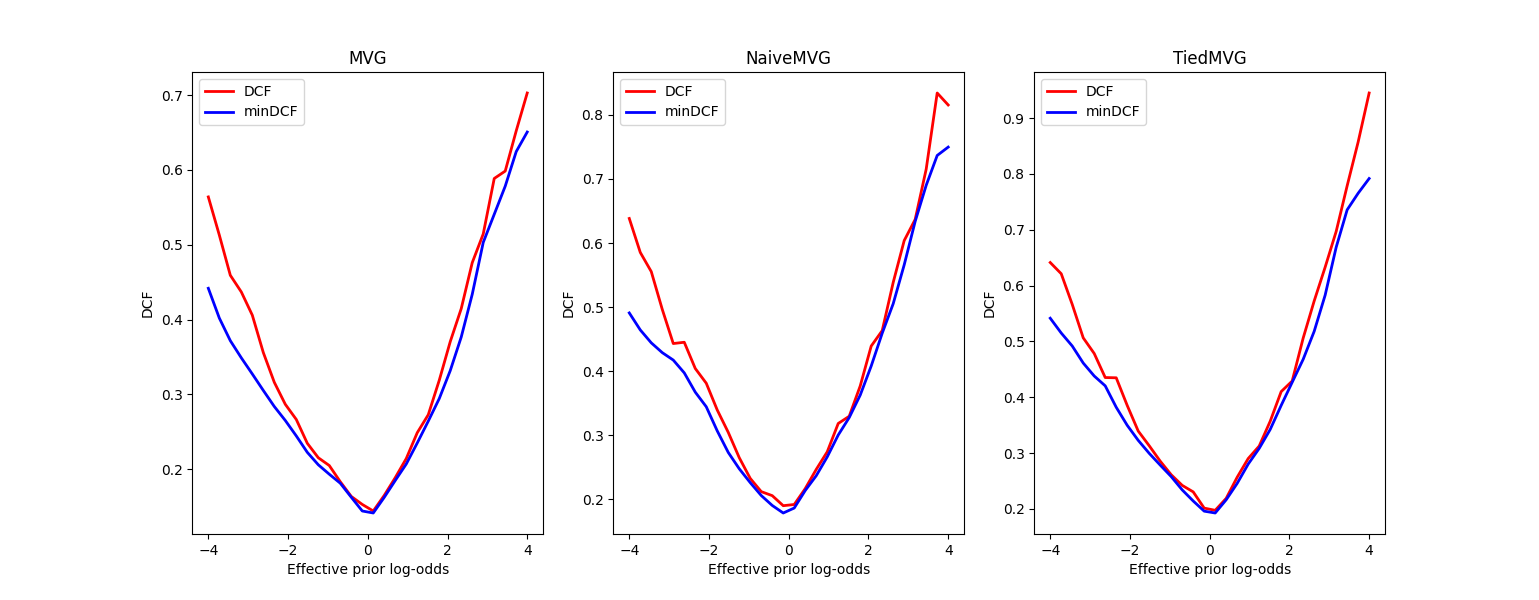
\includegraphics[width=\textwidth]{./plot/MVG/bayes_plot.png}
    \end{subfigure}
    \caption{Bayes error plot for the MVG classifier.}
    \label{fig:bayes_error_MVG}
\end{figure}
\noindent
From this figure we can see that the MVG classifiers are well calibrated in the middle part of the plot, while they show signs of little mis-calibration in the extremes of the plot.

\section{Logistic Regression Classifier}
The second model we are going to use is the binary Logistic Regression (LR) classifier.
\nnl
In the following section we will present the results of the Logistic Regression classifier in terms of DCF and minDCF, using different setups.
\nnl
We will start by using the target application (effective prior = 0.1) and no PCA preprocessing.
\begin{figure}[H]
    \centering
    \begin{subfigure}[t]{0.6\textwidth}
        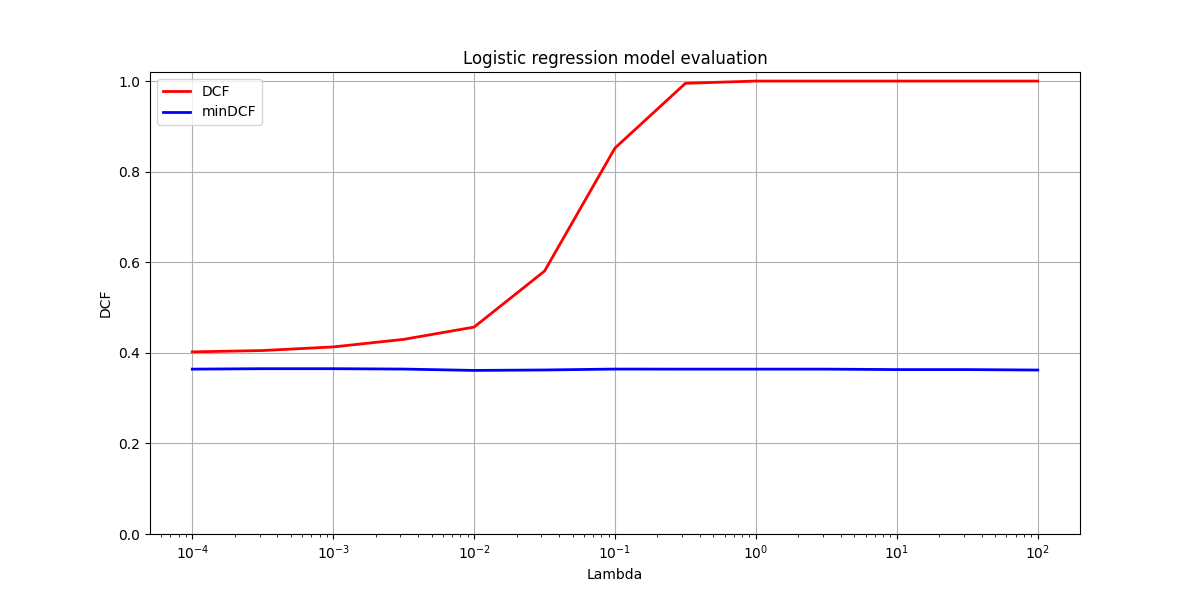
\includegraphics[width=\textwidth]{./plot/LR/log_reg.png}
    \end{subfigure}
    \caption{DCF and minDCF for the Logistic Regression classifier as a function of $\lambda$}
    \label{fig:log_reg}
\end{figure}
\noindent
We observe that the DCF increases with $\lambda$ (the regularization degrades our results), while the minDCF remains quite stable.

\begin{figure}[H]
    \centering
    \begin{subfigure}[t]{0.6\textwidth}
        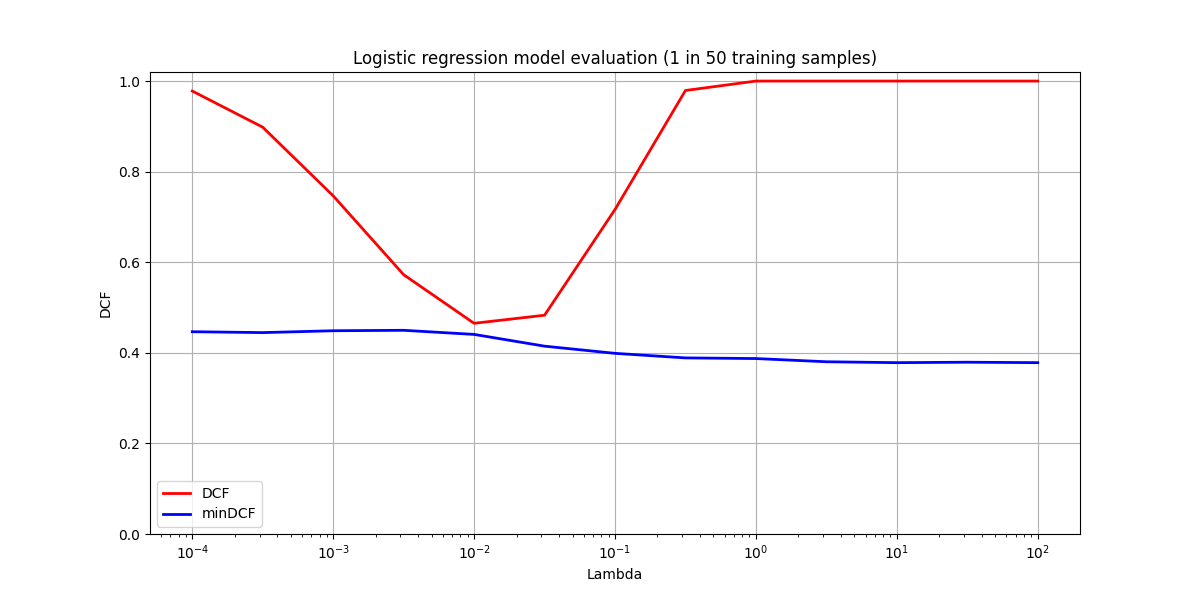
\includegraphics[width=\textwidth]{./plot/LR/log_reg_1in50.png}
    \end{subfigure}
    \caption{DCF and minDCF for the Logistic Regression classifier as a function of $\lambda$ (1 in 50 samples taken)}
    \label{fig:log_reg_1in50}
\end{figure}
\noindent
Removing samples seems to be an effective way to improve the regularization. We can in fact see that now the minDCF decreases with $\lambda$, indicating that the regularization is now effective in improving the classifier.
\nl
Moreover we can see that for $\lambda = 0.01$ our classifier is able to achieve a DCF that is similar to the minDCF, which is a good result.

\begin{figure}[H]
    \centering
    \begin{subfigure}[t]{0.6\textwidth}
        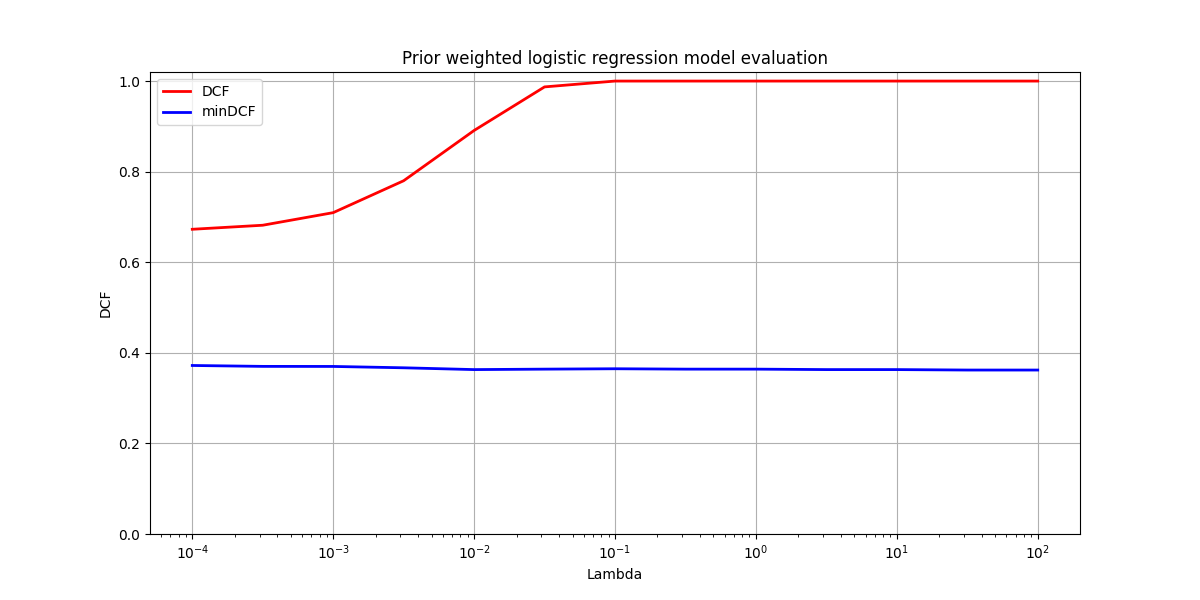
\includegraphics[width=\textwidth]{./plot/LR/prior_w_log_reg.png}
    \end{subfigure}
    \caption{DCF and minDCF for the Prior Weighted Logistic Regression classifier as a function of $\lambda$ (prior = 0.1)}
    \label{fig:pw_log_reg}
\end{figure}
\noindent
We don't observe significant improvements in the minDCF using the prior weighted Logistic Regression classifier. There are though some improvements in the DCF, when using priors like 0.6, 0.7, and 0.8.

\begin{figure}[H]
    \centering
    \begin{subfigure}[t]{0.6\textwidth}
        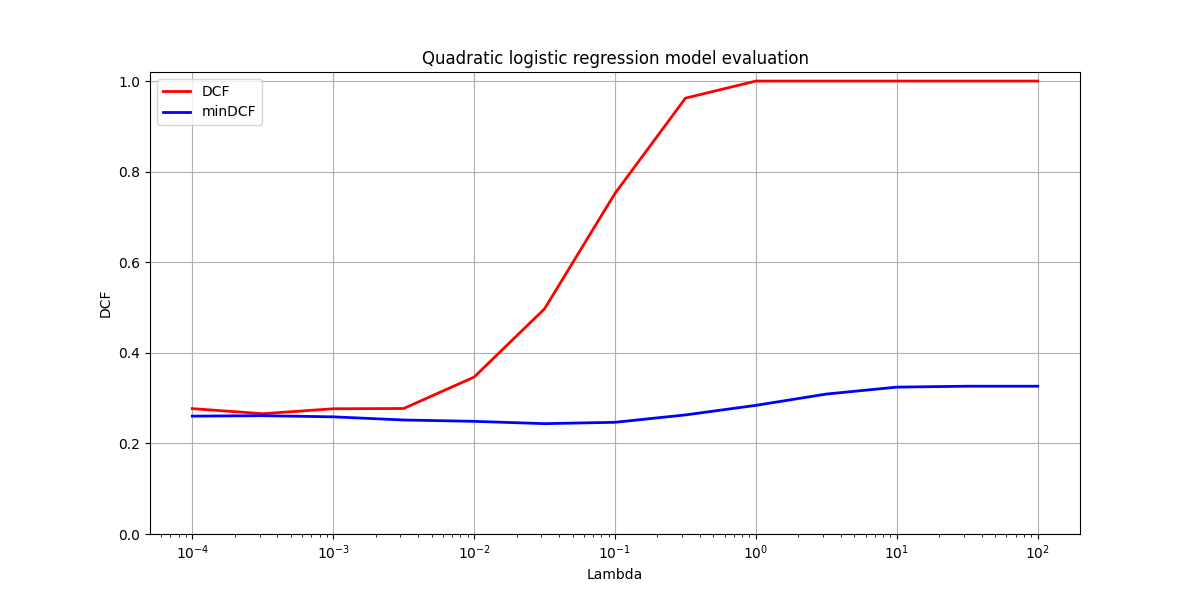
\includegraphics[width=\textwidth]{./plot/LR/quadratic_log_reg.png}
    \end{subfigure}
    \caption{DCF and minDCF for the Quadratic Logistic Regression classifier as a function of $\lambda$}
    \label{fig:qlr}
\end{figure}
\noindent
The Quadratic Logistic Regression classifier is the best model until now in terms of minDCF, with a lowest value of around 0.210 for $\lambda = 0.032$.
\nl
This can be explained by the fact that the Quadratic Logistic Regression classifier is able to model the data in a more complex way, and thus is able to achieve better results.
\nl
We can also see that a "medium" regularization is the best for this model.

\begin{figure}[H]
    \centering
    \begin{subfigure}[t]{0.32\textwidth}
        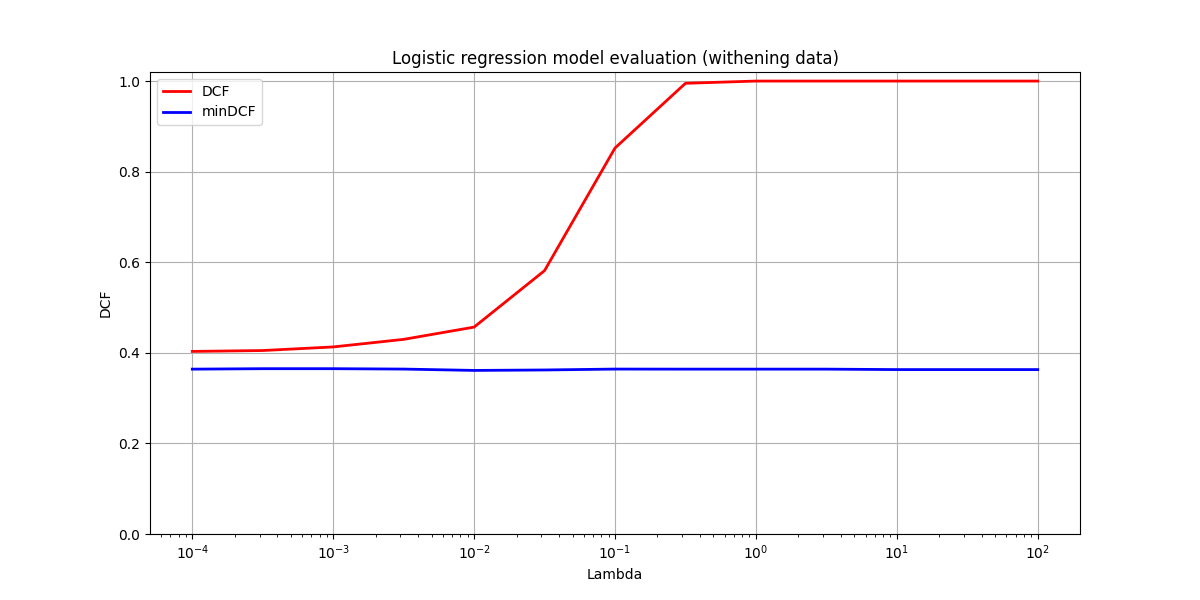
\includegraphics[width=\textwidth]{./plot/LR/log_reg_withening.png}
    \end{subfigure}
    \hfill
    \begin{subfigure}[t]{0.32\textwidth}
        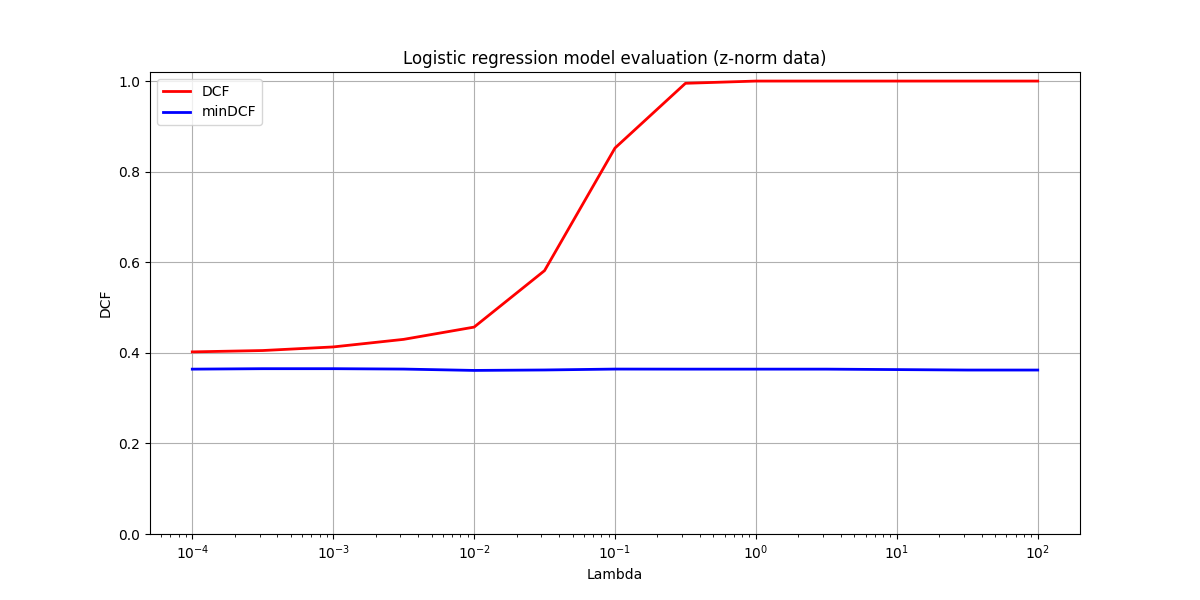
\includegraphics[width=\textwidth]{./plot/LR/log_reg_znorm.png}
    \end{subfigure}
    \hfill
    \begin{subfigure}[t]{0.32\textwidth}
        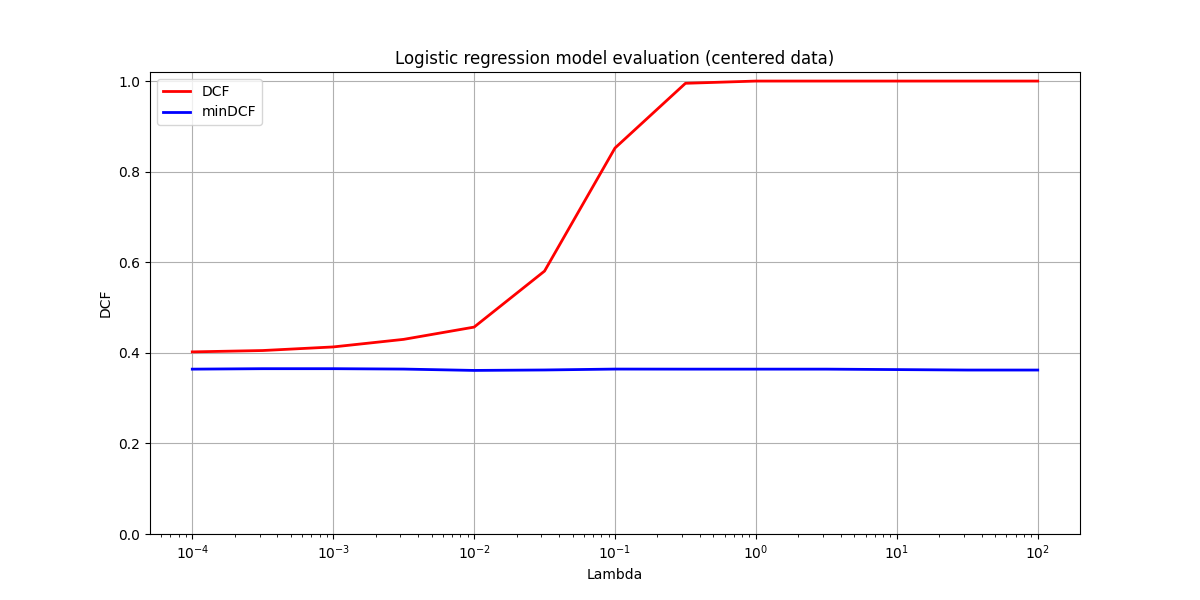
\includegraphics[width=\textwidth]{./plot/LR/log_reg_centered.png}
    \end{subfigure}
    \caption{DCF and minDCF for the Logistic Regression classifier with different preprocessing steps.}
    \label{fig:log_reg_preprocessing}
\end{figure}
\noindent
In these plots we can see that using techniques like whitening, z-normalization, and centering on the standard LR model doesn't improve the performances.
\nl
This is probably due to the fact that the original data is already well scaled and centered.
\nnl
As a final step we will try to classify the samples using PCA as a preprocessing step.

\begin{figure}[H]
    \centering
    \begin{subfigure}[t]{0.32\textwidth}
        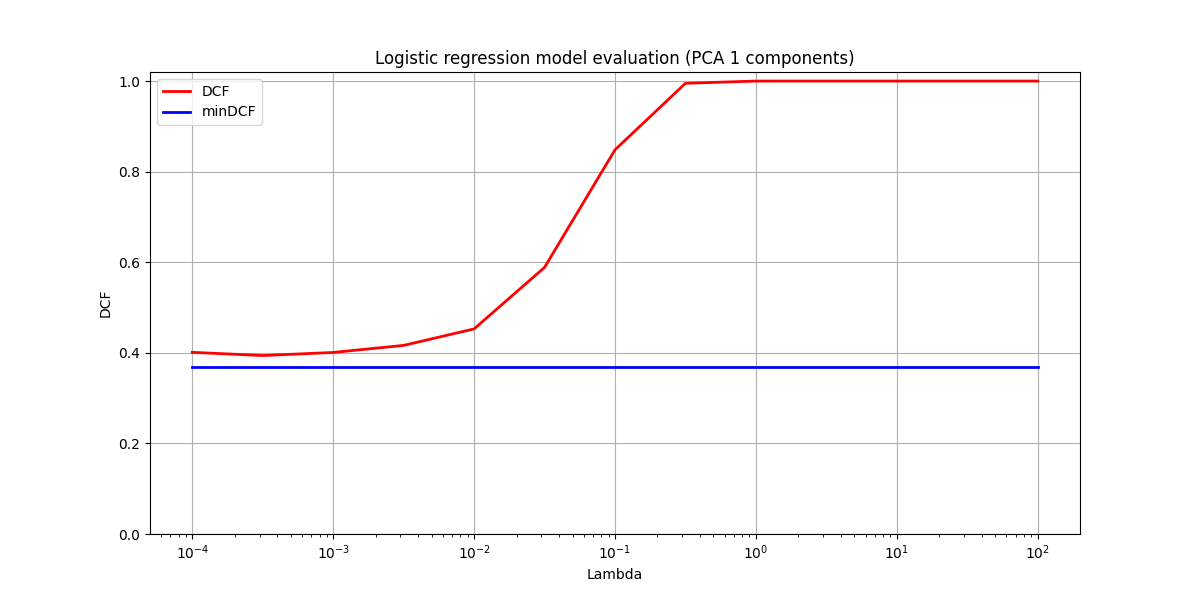
\includegraphics[width=\textwidth]{./plot/LR/log_reg_pca1.png}
    \end{subfigure}
    \hfill
    \begin{subfigure}[t]{0.32\textwidth}
        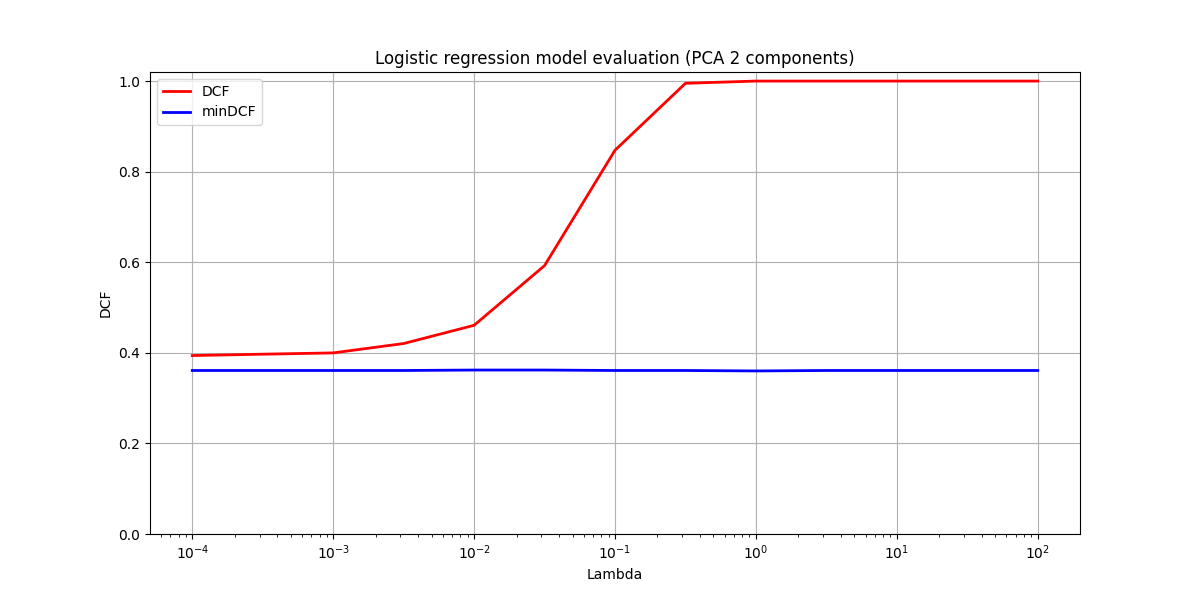
\includegraphics[width=\textwidth]{./plot/LR/log_reg_pca2.png}
    \end{subfigure}
    \hfill
    \begin{subfigure}[t]{0.32\textwidth}
        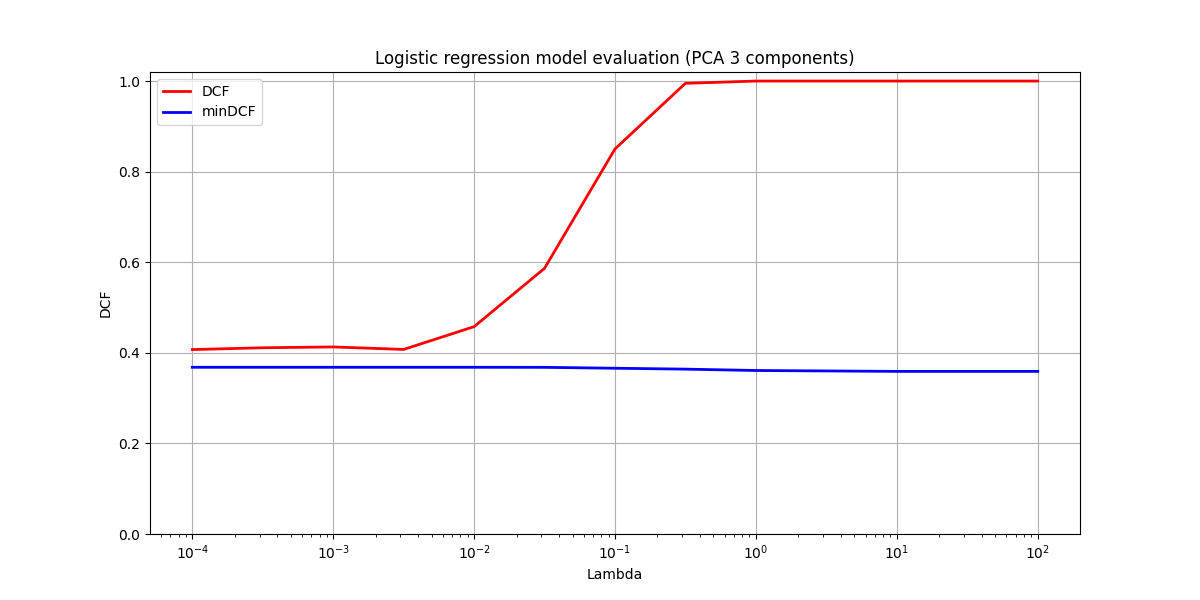
\includegraphics[width=\textwidth]{./plot/LR/log_reg_pca3.png}
    \end{subfigure}
    %%%%%%%%%%%%%%%%%%%%%%%%%%%%%%%%%%%%second row
    \begin{subfigure}[t]{0.32\textwidth}
        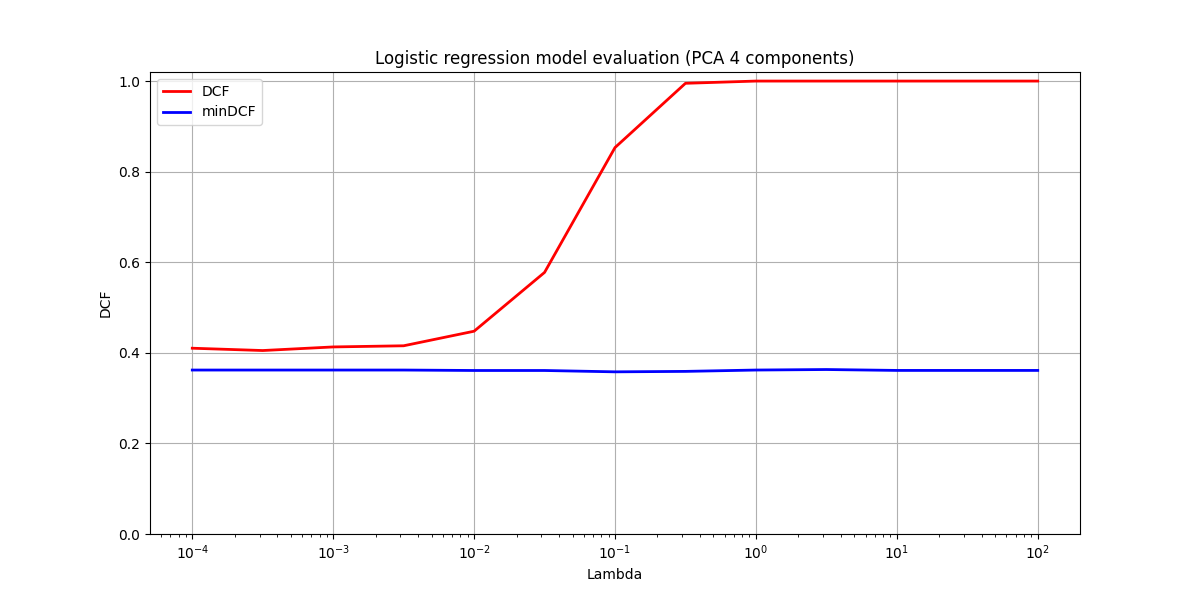
\includegraphics[width=\textwidth]{./plot/LR/log_reg_pca4.png}
    \end{subfigure}
    \hfill
    \begin{subfigure}[t]{0.32\textwidth}
        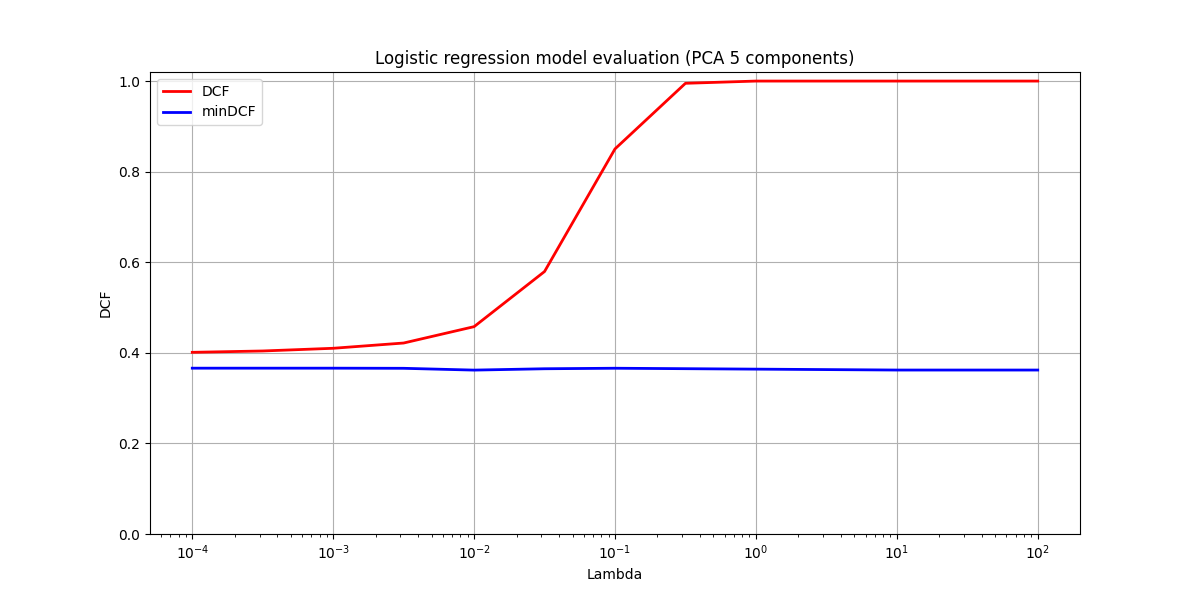
\includegraphics[width=\textwidth]{./plot/LR/log_reg_pca5.png}
    \end{subfigure}
    \hfill
    \begin{subfigure}[t]{0.32\textwidth}
        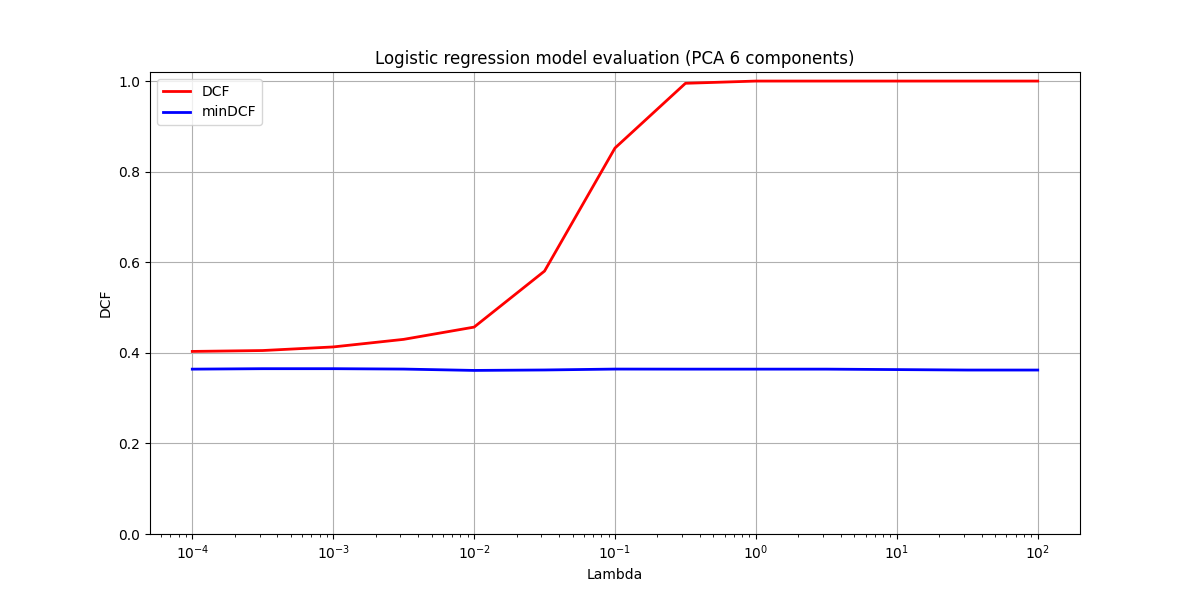
\includegraphics[width=\textwidth]{./plot/LR/log_reg_pca6.png}
    \end{subfigure}

    \caption{DCF and minDCF for the Logistic Regression classifier with PCA preprocessing.}
    \label{fig:log_reg_pca}
\end{figure}
\noindent
We can see that also in this case PCA doesn't seem to be effective in improving the performances of the Logistic Regression classifier.
\nnl
We can end our analysis of the Logistic Regression classifier by observing that all the different approach that we have used suffer from the same problem: heavy mis-calibration.
\nnl
Moreover we can see that, up to now, the Quadratic Logistic Regression classifier is the best model in terms of minDCF, with a value of around 0.210, beating the MVG classifier with the best setup (0.263).
\nl
The gap in performances can be explained by the fact that the Quadratic Logistic Regression classifier is able to model the data that is not linearly separable in a better way than the MVG classifier. Observing the scatter plots of the features we can see that most of them are not linearly separable, thus the Quadratic Logistic Regression classifier is able to achieve better results.

\section{Support Vector Machine Classifier}
The third model we are going to use is the Support Vector Machine (SVM) classifier.
\nl
This is a powerful model that is able to classify samples both in a linear and non-linear way (with the use of the kernel trick).
\nnl
We will start with the simple SVM classifier and then we will use the SVM with polynomial and RBF kernels.

\begin{figure}[H]
    \centering
    \begin{subfigure}[t]{0.6\textwidth}
        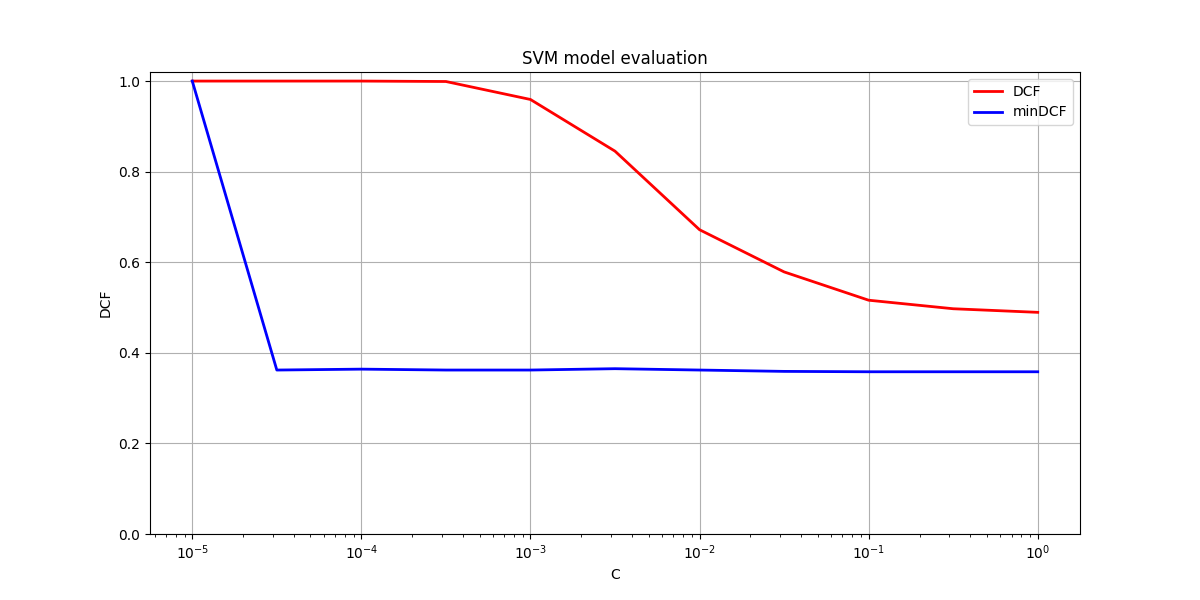
\includegraphics[width=\textwidth]{./plot/SVM/svm.png}
    \end{subfigure}
    \caption{DCF and minDCF for the SVM classifier as a function of the regularization parameter.}
    \label{fig:svm}
\end{figure}
\noindent
As we can see the results obtained by this model are not good compared to the other models. This is another strong indication that the data is not linearly separable.
\nl
Moreover in this case lower regularization is better (high values of the parameter C), indicating that the model is not overfitting the data. Both the DCF and minDCF decrease with the regularization parameter.

\begin{figure}[H]
    \centering
    \begin{subfigure}[t]{0.6\textwidth}
        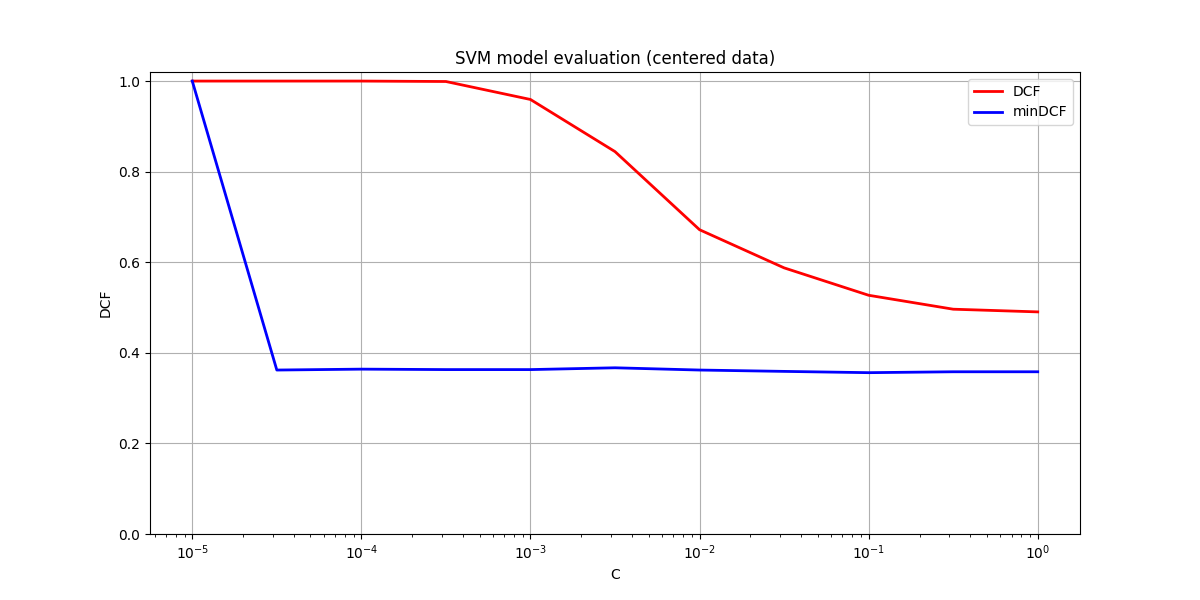
\includegraphics[width=\textwidth]{./plot/SVM/svm_centered.png}
    \end{subfigure}
    \caption{DCF and minDCF for the SVM classifier as a function of the regularization parameter (centered data).}
    \label{fig:svm_centered}
\end{figure}
\noindent
Centering the data doesn't seem to improve the performances of the SVM classifier. The results are similar to the ones obtained with the original data, confirming that the data is already well centered.
\nl
The same can be said about the regularization parameter: the best results are obtained with low regularization.

\begin{figure}[H]
    \centering
    \begin{subfigure}[t]{0.6\textwidth}
        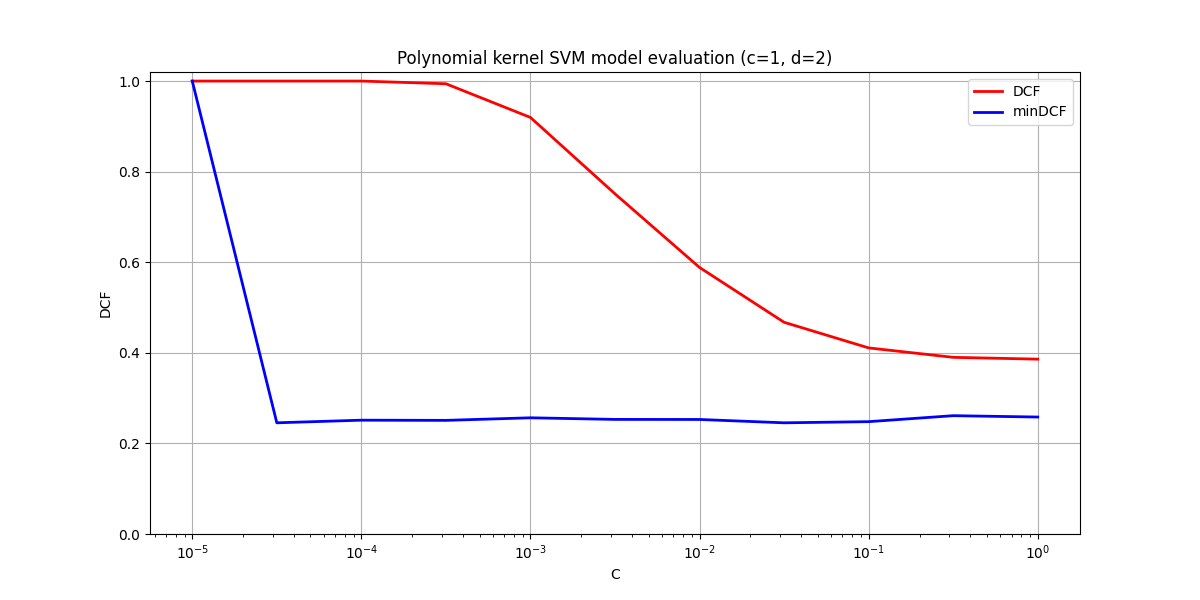
\includegraphics[width=\textwidth]{./plot/SVM/svm_poly.png}
    \end{subfigure}
    \caption{DCF and minDCF for the SVM with polynomial kernel classifier as a function of the regularization parameter.}
    \label{fig:svm_poly}
\end{figure}
\noindent
The SVM with polynomial kernel is able to achieve better results than the simple SVM classifier. We can see a huge improvement in the minDCF, which is now around 0.210 for the best setup.
\nl
Here we used a polynomial kernel of degree 2, which is able to model the data in a better way than the linear kernel.
\nl
The low regularization trend is confirmed also in this case.

\begin{figure}[H]
    \centering
    \begin{subfigure}[t]{0.6\textwidth}
        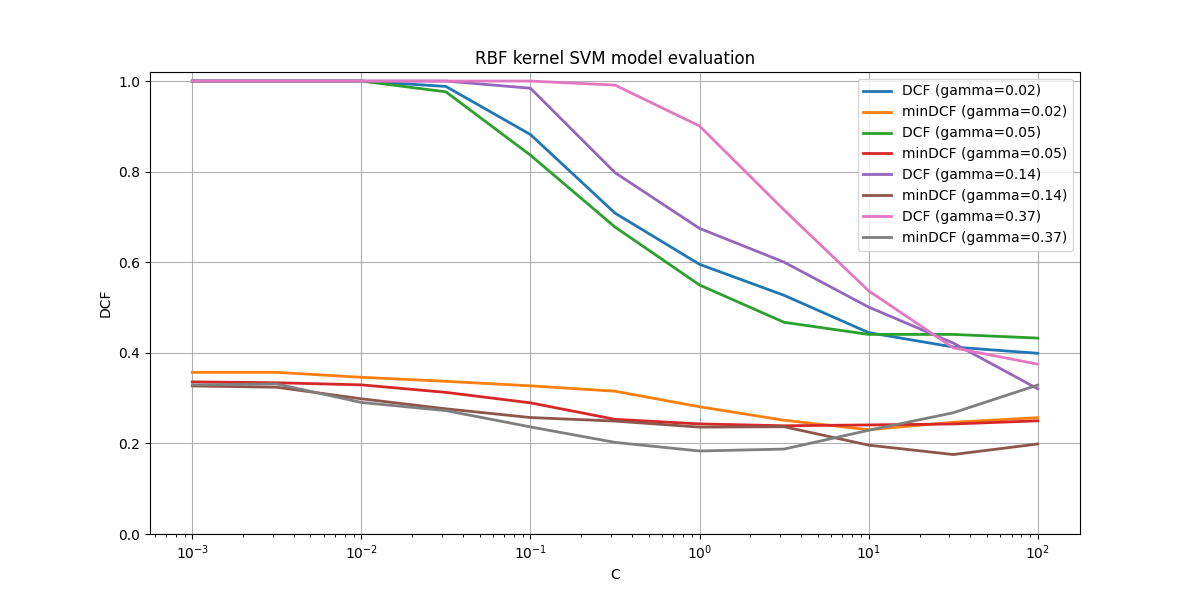
\includegraphics[width=\textwidth]{./plot/SVM/svm_rbf.png}
    \end{subfigure}
    \caption{DCF and minDCF for the SVM classifier with RBF kernel as a function of the regularization parameter.}
    \label{fig:svm_rbf}
\end{figure}
\noindent
Using the RBF kernel we are able to achieve the best results until now. The minDCF is lower than 0.200 for the best setup, which is the best result obtained until now.
\nl
This can be explained by the fact that the RBF kernel is able to model the data in a more complex way, confirming again the non linear separability of the data.
\nnl
To conclude the analysis of the SVM classifier we can say that the best model is the SVM with RBF kernel, with the best setup being $C=32$ and $\gamma=0.135$.
\nl
Moreover all the models suffer from mis-calibration, and they would greatly benefit from a calibration step.

\section{Gaussian Mixture Model Classifier}
The fourth and last model we are going to use is the Gaussian Mixture Model (GMM) classifier.
\nnl
In the following we present the results of the GMM classifier in terms of DCF and minDCF, using different setups.

\begin{figure}[H]
    \centering
    \begin{subfigure}[t]{0.6\textwidth}
        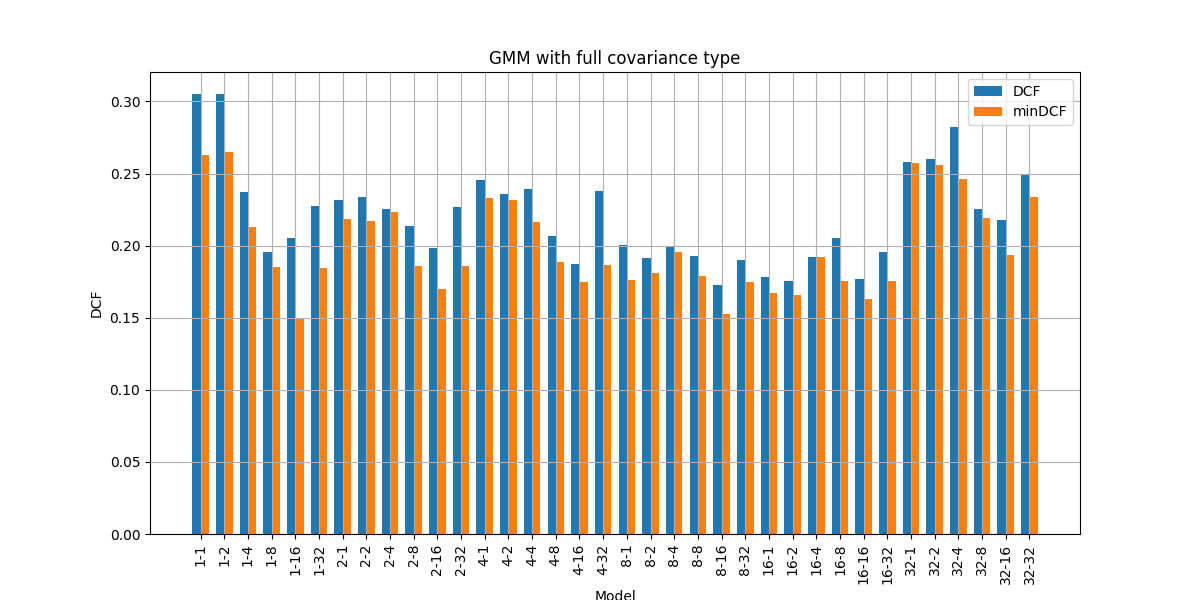
\includegraphics[width=\textwidth]{./plot/GMM/gmm_full.png}
    \end{subfigure}
    \caption{DCF and minDCF for the GMM classifier as a function of the number of components.}
    \label{fig:gmm}
\end{figure}

\begin{figure}[H]
    \centering
    \begin{subfigure}[t]{0.6\textwidth}
        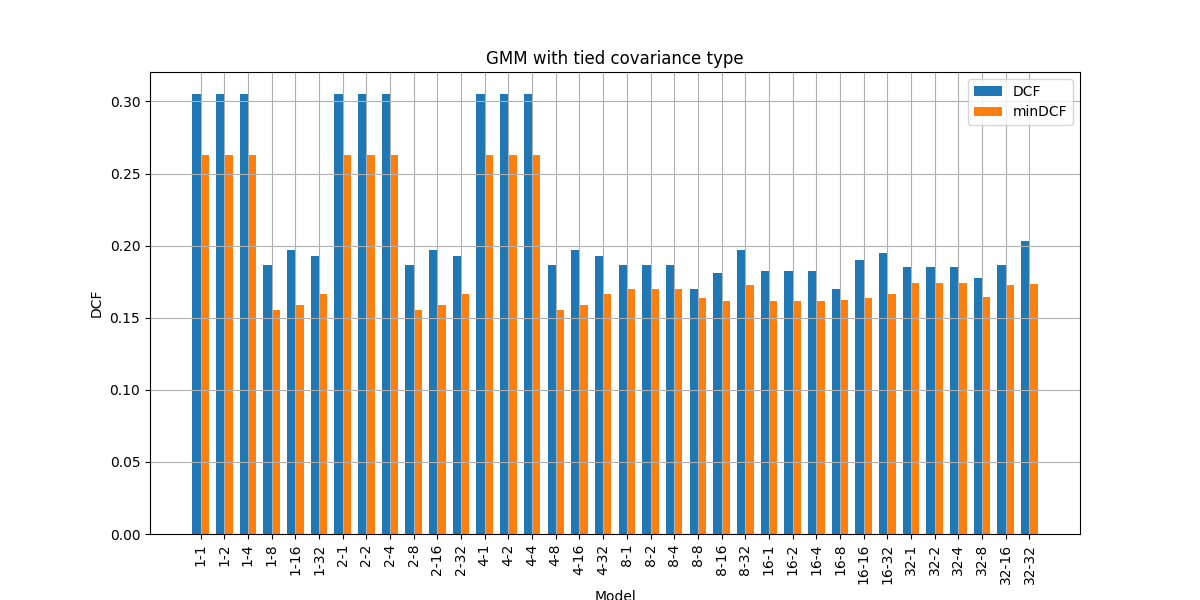
\includegraphics[width=\textwidth]{./plot/GMM/gmm_tied.png}
    \end{subfigure}
    \caption{DCF and minDCF for the GMM (tied covariance matrix) classifier as a function of the number of components.}
    \label{fig:gmm_tied}
\end{figure}

\begin{figure}[H]
    \centering
    \begin{subfigure}[t]{0.6\textwidth}
        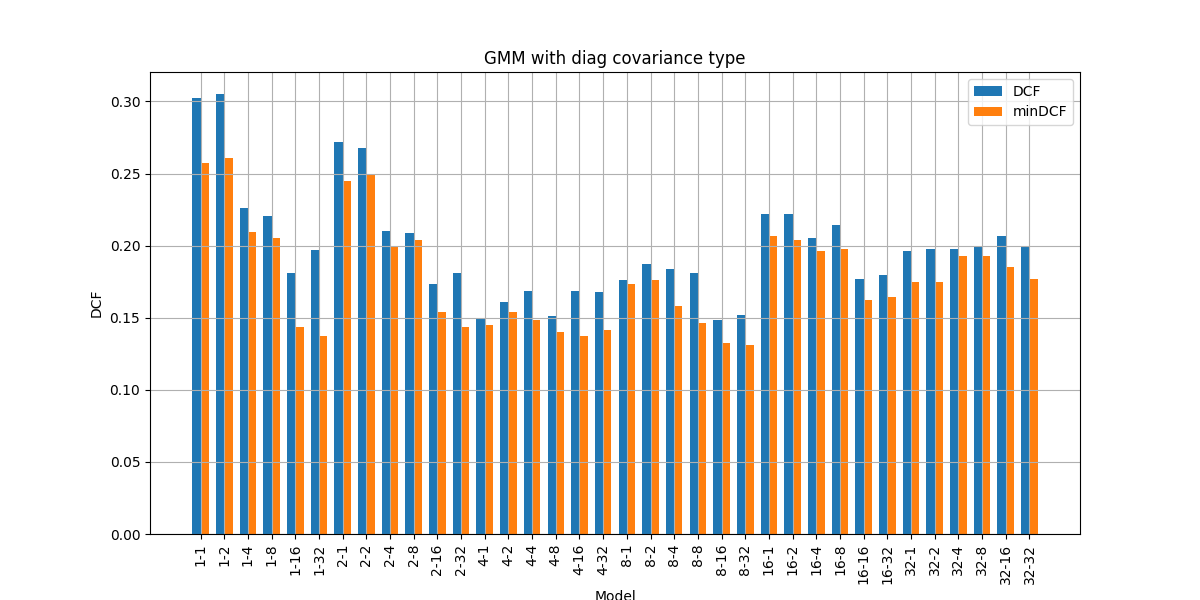
\includegraphics[width=\textwidth]{./plot/GMM/gmm_diag.png}
    \end{subfigure}
    \caption{DCF and minDCF for the GMM (diagonal covariance matrix) classifier as a function of the number of components.}
    \label{fig:gmm_diag}
\end{figure}
\noindent
The GMM classifier is in general able to achieve good results. We could have expected this since GMM is a more complex model than the other models we have used, and as we said before is a good candidate to model some of the features of our dataset.
\nnl
The best results are obtained with the diagonal covariance matrix GMM with 8 components for class 0 and 32 components for class 1. The minDCF is around 0.130, which is the best result obtained until this moment.
\nl
These results are in line with the analysis we have done. In particular we have seen that the data is not linearly separable, and that the features are not correlated (even tough in the diagonal covariance matrix case we are doing a different assumption wrt to the Naive assumption).

\section{Model Comparison}
We can now compare the models in terms of minDCF, to see which one is the best model for our dataset.
\nnl
In this section we will take the best candidates for each model and compare them in terms of minDCF.
\nl
The three best models that we will consider are:
\begin{itemize}
    \item Quadratic Logistic Regression classifier ($\lambda = 0.032$)
    \item SVM with RBF kernel ($C=32$, $\gamma=0.135$)
    \item GMM with diagonal covariance matrix (8 components for class 0, 32 components for class 1)
\end{itemize}
We will plot the Bayes error plots and analyze them.

\begin{figure}[H]
    \centering
    \begin{subfigure}[t]{0.6\textwidth}
        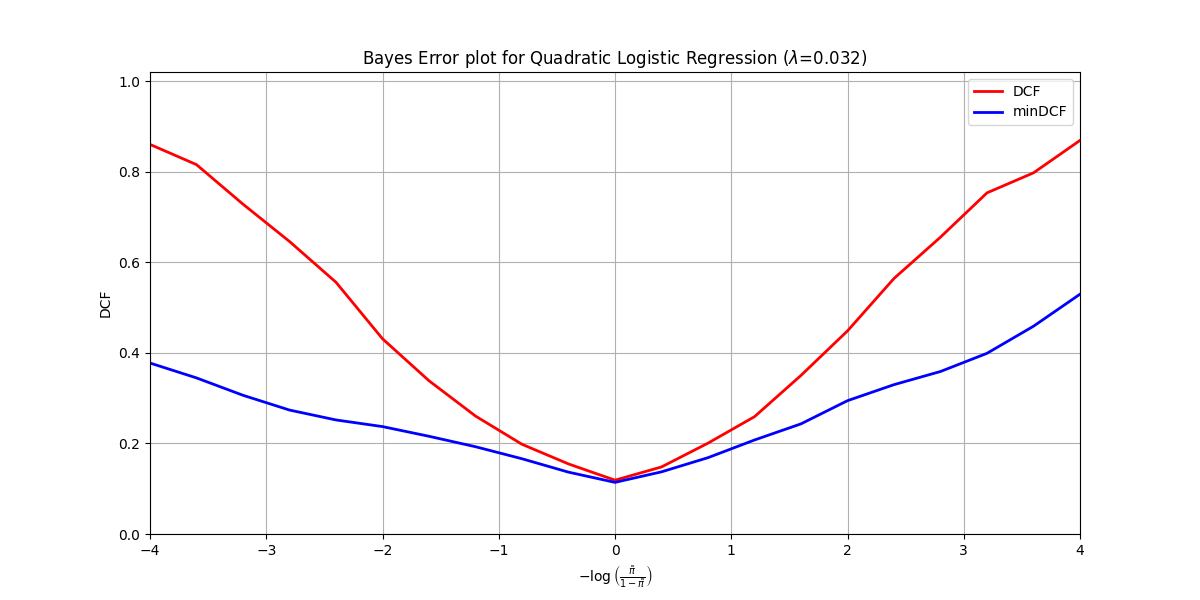
\includegraphics[width=\textwidth]{./plot/model_selection/LogisticRegression.png}
    \end{subfigure}
    \caption{Bayes error plot for the Quadratic Logistic Regression classifier.}
    \label{fig:bayes_error_LR}
\end{figure}

\begin{figure}[H]
    \centering
    \begin{subfigure}[t]{0.6\textwidth}
        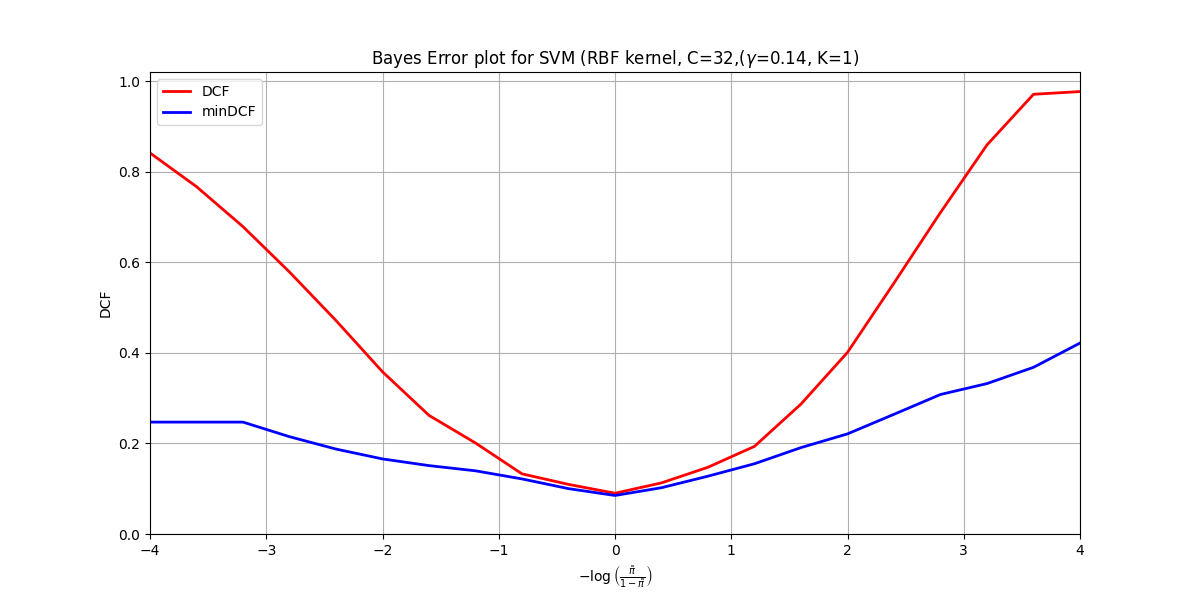
\includegraphics[width=\textwidth]{./plot/model_selection/kernelSVM.png}
    \end{subfigure}
    \caption{Bayes error plot for the SVM with RBF kernel classifier.}
    \label{fig:bayes_error_SVM}
\end{figure}

\begin{figure}[H]
    \centering
    \begin{subfigure}[t]{0.6\textwidth}
        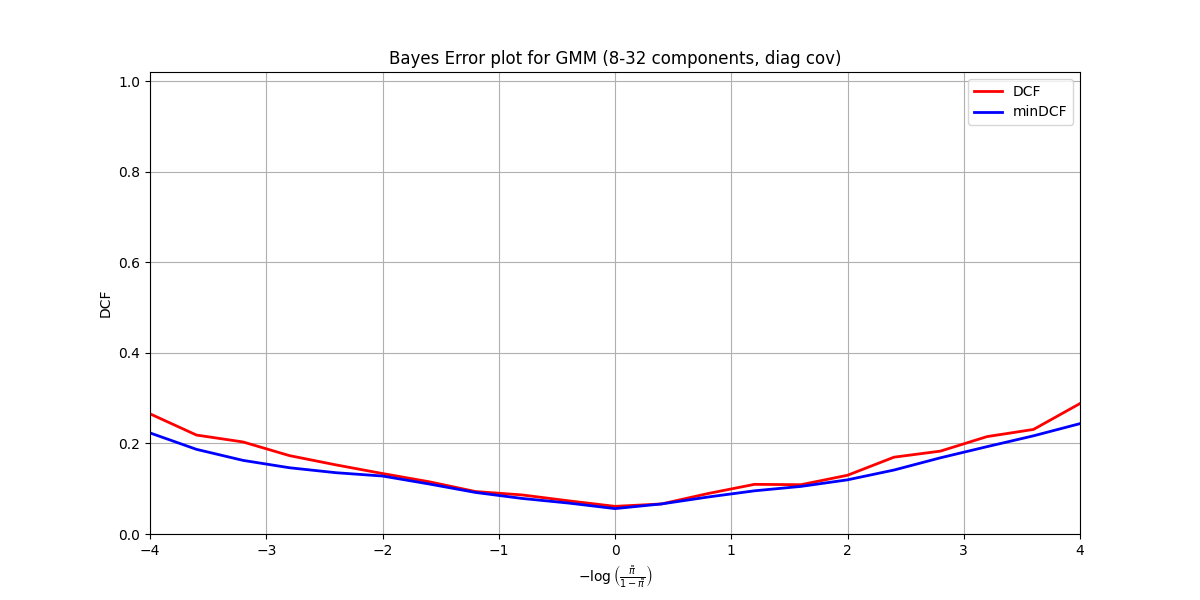
\includegraphics[width=\textwidth]{./plot/model_selection/GMM.png}
    \end{subfigure}
    \caption{Bayes error plot for the GMM with diagonal covariance matrix classifier.}
    \label{fig:bayes_error_GMM}
\end{figure}
\noindent
We can see that the relative ranking of the models is preserved even if we consider other priors: the GMM classifier is the best model, followed by the SVM with RBF kernel, and then the Quadratic Logistic Regression classifier.
\nnl
We can also observe that the SVM model and the QLR model are not well calibrated, while the GMM model is well calibrated across the whole range of priors.
\nl
In particular these models (SVM and QLR) harm priors that are not close to 0.5. This is an important consideration since our application has a prior of 0.1.

\section{Score Calibration}
As we have seen in the previous sections, the models we have used are not well calibrated. This is a problem since the DCF is a metric that is sensitive to the calibration of the models.
\nl
This is due to the fact that until now we have used as threshold the theoretical threshold ($-{log}\frac{\pi}{1-\pi}$) that is not always optimal. That's why we see huge differences in the DCF and minDCF values, especially for our target application.
\nnl
In this section we will try to calibrate the models using the Prior Weighted Logistic Regression as a calibration model. We will use a 5-fold cross validation to calibrate the models.
\subsubsection*{Quadratic Logistic Regression}
We will start by calibrating the Quadratic Logistic Regression classifier.

\begin{figure}[H]
    \centering
    \begin{subfigure}[t]{0.6\textwidth}
        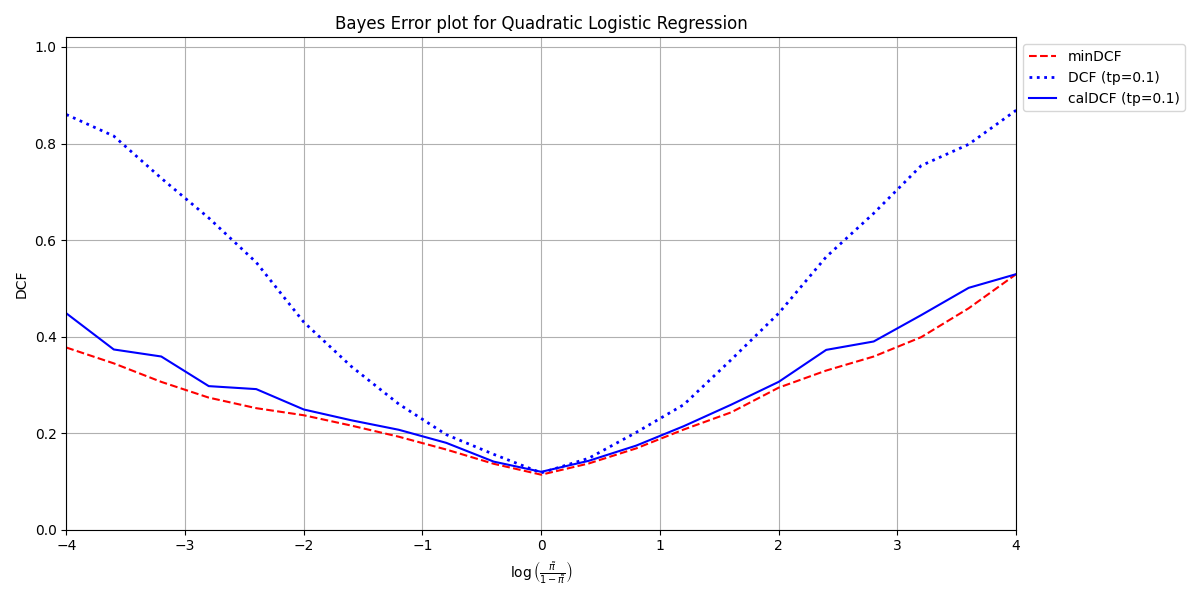
\includegraphics[width=\textwidth]{./plot/calibration/QLR.png}
    \end{subfigure}
    \caption{Calibration of the Quadratic Logistic Regression classifier (training prior = 0.1).}
    \label{fig:calibration_QLR}
\end{figure}
\noindent
As we can see in this figure the calibration is able to drastically improve the performances of the model over the whole range of priors.
\nl
In the figure we have reported the calibration for a training prior of 0.1, but we have also tried different training priors and the results were similar.
\nnl
In the following table we instead report the minDCF, DCF, and calDCF for different training priors, considering our target application (effective prior = 0.1).
\begin{table}[H]
    \centering
    \begin{tabular}{|c|c|c|c|}
        \hline
        \rowcolor{blue!10}
        \textbf{Training Prior} & \textbf{minDCF} & \textbf{DCF} & \textbf{calDCF}                  \\
        \hline
        0.1                     & 0.244           & 0.496        & 0.268                            \\
        \hline
        0.2                     & 0.244           & 0.496        & 0.265                            \\
        \hline
        0.3                     & 0.244           & 0.496        & 0.276                            \\
        \hline
        0.4                     & 0.244           & 0.496        & 0.251                            \\
        \hline
        0.5                     & 0.244           & 0.496        & 0.281                            \\
        \hline
        0.6                     & 0.244           & 0.496        & 0.254                            \\
        \hline
        0.7                     & 0.244           & 0.496        & \textcolor{cyan}{\textbf{0.248}} \\
        \hline
        0.8                     & 0.244           & 0.496        & 0.258                            \\
        \hline
        0.9                     & 0.244           & 0.496        & 0.256                            \\
        \hline
    \end{tabular}
    \caption{Quadratic Logistic Regression: minDCF, DCF, and calDCF for different training priors}
    \label{tab:QLR_Priors}
\end{table}
\noindent
We obtain the best results for training priors of 0.7, with a calDCF of 0.248.
\subsubsection*{SVM with RBF Kernel}
\begin{figure}[H]
    \centering
    \begin{subfigure}[t]{0.6\textwidth}
        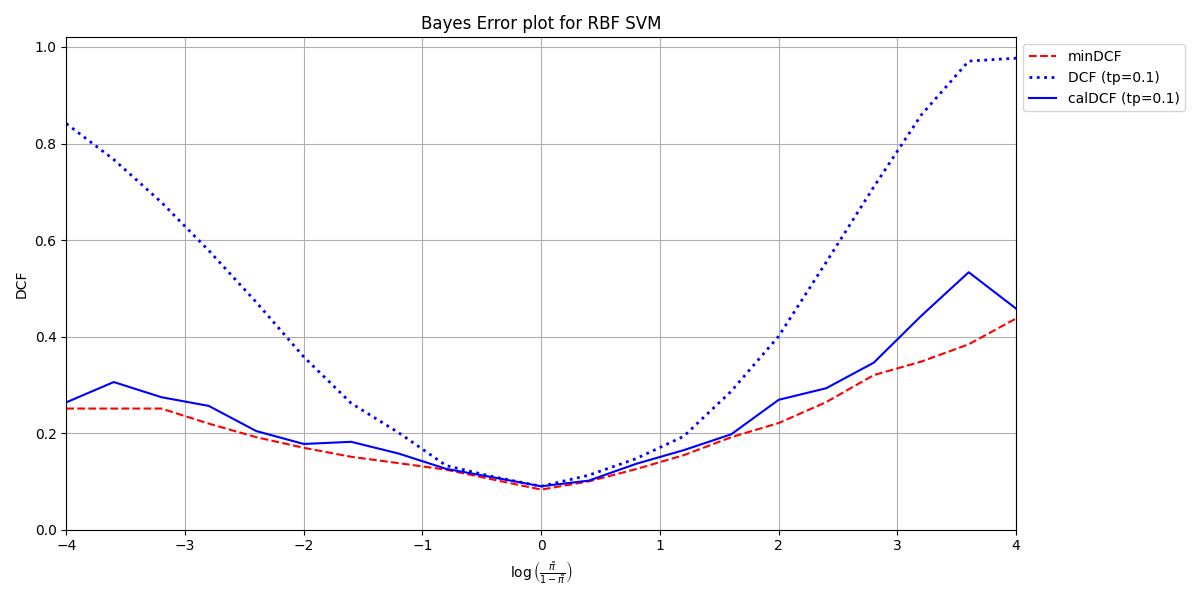
\includegraphics[width=\textwidth]{./plot/calibration/RBF_SVM.png}
    \end{subfigure}
    \caption{Calibration of the SVM with RBF kernel classifier (training prior = 0.1).}
    \label{fig:calibration_SVM}
\end{figure}
\noindent
Following the same approach as before, we have plotted the bayes error plot for the SVM with RBF kernel. We can see that the calibration is able to improve the performances of the model, especially in the extremes of the plot.
\begin{table}[H]
    \centering
    \begin{tabular}{|c|c|c|c|}
        \hline
        \rowcolor{blue!10}
        \textbf{Training Prior} & \textbf{minDCF} & \textbf{DCF} & \textbf{calDCF}                  \\
        \hline
        0.1                     & 0.175           & 0.422        & \textcolor{cyan}{\textbf{0.179}} \\
        \hline
        0.2                     & 0.175           & 0.422        & 0.181                            \\
        \hline
        0.3                     & 0.175           & 0.422        & 0.186                            \\
        \hline
        0.4                     & 0.175           & 0.422        & 0.188                            \\
        \hline
        0.5                     & 0.175           & 0.422        & 0.200                            \\
        \hline
        0.6                     & 0.175           & 0.422        & 0.194                            \\
        \hline
        0.7                     & 0.175           & 0.422        & 0.193                            \\
        \hline
        0.8                     & 0.175           & 0.422        & 0.197                            \\
        \hline
        0.9                     & 0.175           & 0.422        & 0.208                            \\
        \hline
    \end{tabular}
    \caption{RBF SVM: minDCF, DCF, and calDCF for different training priors}
    \label{tab:RBF_SVM_Priors}
\end{table}
\noindent
Here we obtain the best results for a training prior of 0.1, with a calDCF of 0.179.
\subsubsection*{GMM}
\begin{figure}[H]
    \centering
    \begin{subfigure}[t]{0.6\textwidth}
        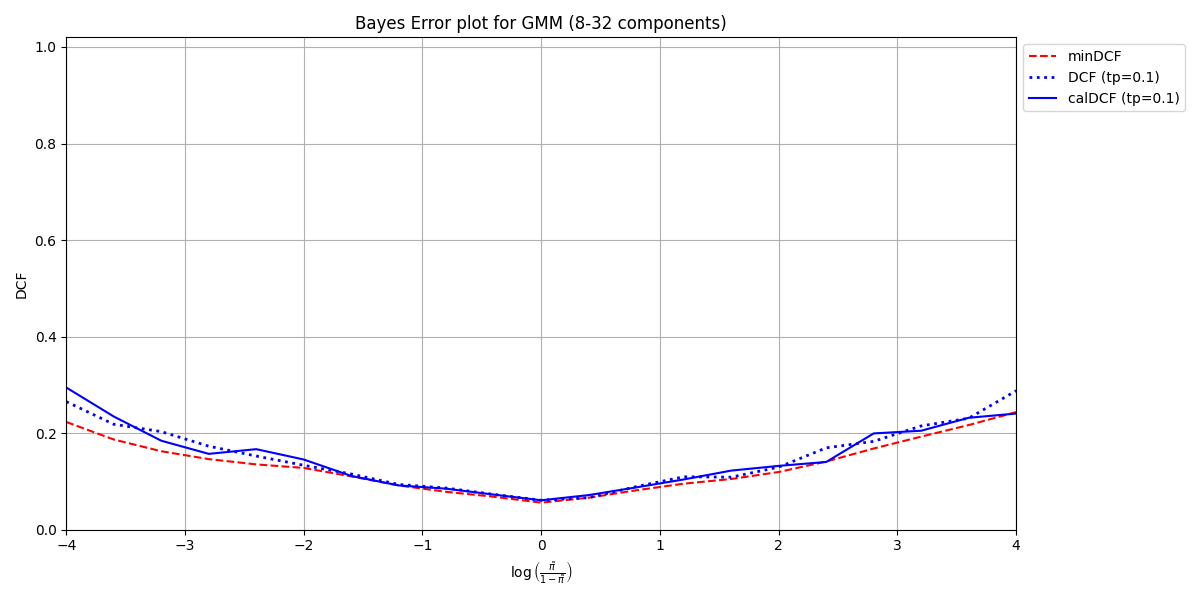
\includegraphics[width=\textwidth]{./plot/calibration/GMM.png}
    \end{subfigure}
    \caption{Calibration of the GMM with diagonal covariance matrix classifier (training prior = 0.1).}
    \label{fig:calibration_GMM}
\end{figure}
\noindent
Finally we have calibrated the GMM classifier. We can see that the original model was already well calibrated, and the calibration step didn't improve the performances of the model by much. For some priors the calibration step even worsened the performances of the model.
\begin{table}[H]
    \centering
    \begin{tabular}{|c|c|c|c|}
        \hline
        \rowcolor{blue!10}
        \textbf{Training Prior} & \textbf{minDCF} & \textbf{DCF} & \textbf{calDCF}                  \\
        \hline
        0.1                     & 0.131           & 0.152        & 0.162                            \\
        \hline
        0.2                     & 0.131           & 0.152        & 0.150                            \\
        \hline
        0.3                     & 0.131           & 0.152        & 0.154                            \\
        \hline
        0.4                     & 0.131           & 0.152        & 0.154                            \\
        \hline
        0.5                     & 0.131           & 0.152        & 0.150                            \\
        \hline
        0.6                     & 0.131           & 0.152        & 0.152                            \\
        \hline
        0.7                     & 0.131           & 0.152        & 0.160                            \\
        \hline
        0.8                     & 0.131           & 0.152        & 0.159                            \\
        \hline
        0.9                     & 0.131           & 0.152        & \textcolor{cyan}{\textbf{0.148}} \\
        \hline
    \end{tabular}
    \caption{GMM (8-32 components): minDCF, DCF, and calDCF for different training priors}
    \label{tab:GMM_Priors}
\end{table}
\noindent
Here we obtain the best results for a training prior of 0.9, with a calDCF of 0.148.
\nnl
Even after the calibration step the GMM classifier is the best model, followed by the SVM with RBF kernel, and then the Quadratic Logistic Regression classifier.

\section{Model Fusion}
In this section we will try to fuse the models we have used in order to improve the performances of the classifiers.
\nl
We will use a technique called "score fusion" that is able to combine the scores of the models in order to obtain a better classification.
\nnl
Here are the results of the fused models in terms of minDCF, DCF for our target application (effective prior = 0.1).
\begin{table}[H]
    \centering
    \begin{tabular}{|c|c|c|}
        \hline
        \rowcolor{blue!10}
        \textbf{Model}      & \textbf{minDCF}                  & \textbf{DCF}            \\
        \hline
        QLR + RBF SVM       & 0.216                            & 0.459                   \\
        \hline
        QLR + GMM           & 0.217                            & 0.324                   \\
        \hline
        RBF SVM + GMM       & \textcolor{cyan}{\textbf{0.185}} & \textcolor{cyan}{0.287} \\
        \hline
        QLR + RBF SVM + GMM & 0.214                            & 0.356                   \\
        \hline
    \end{tabular}
    \caption{Fused models: minDCF and DCF for different combinations of models}
    \label{tab:Fused_Models}
\end{table}
\noindent
We can see that the best model is the one that fuses the RBF SVM and the GMM classifier, with a minDCF of 0.185. We can observe that also this fused model suffers from mis-calibration (the DCF is quite higher than the minDCF for our target application).
\nnl
Again, we applied score calibration with different priors for the training of the calibration model, and presented the results in the following tables.

\begin{table}[H]
    \centering
    \begin{tabular}{|c|c|c|}
        \hline
        \rowcolor{blue!10}
        \textbf{Training Prior} & \textbf{minDCF} & \textbf{calDCF}                  \\
        \hline
        0.1                     & 0.179           & 0.200                            \\
        \hline
        0.2                     & 0.175           & 0.198                            \\
        \hline
        0.3                     & 0.177           & 0.195                            \\
        \hline
        0.4                     & 0.174           & 0.200                            \\
        \hline
        0.5                     & 0.177           & 0.204                            \\
        \hline
        0.6                     & 0.172           & 0.196                            \\
        \hline
        0.7                     & 0.181           & 0.198                            \\
        \hline
        0.8                     & 0.178           & 0.197                            \\
        \hline
        0.9                     & 0.175           & \textcolor{cyan}{\textbf{0.191}} \\
        \hline
    \end{tabular}
    \caption{QLR + RBF SVM: minDCF, DCF, and calDCF for different training priors}
    \label{tab:QLR_RBF_SVM_Priors}
\end{table}

\begin{table}[H]
    \centering
    \begin{tabular}{|c|c|c|}
        \hline
        \rowcolor{blue!10}
        \textbf{Training Prior} & \textbf{minDCF} & \textbf{calDCF}                  \\
        \hline
        0.1                     & 0.124           & 0.162                            \\
        \hline
        0.2                     & 0.129           & 0.145                            \\
        \hline
        0.3                     & 0.127           & \textcolor{cyan}{\textbf{0.144}} \\
        \hline
        0.4                     & 0.135           & 0.155                            \\
        \hline
        0.5                     & 0.136           & 0.150                            \\
        \hline
        0.6                     & 0.133           & 0.152                            \\
        \hline
        0.7                     & 0.132           & 0.151                            \\
        \hline
        0.8                     & 0.126           & 0.151                            \\
        \hline
        0.9                     & 0.147           & 0.157                            \\
        \hline
    \end{tabular}
    \caption{QLR + GMM: minDCF, DCF, and calDCF for different training priors}
    \label{tab:QLR_GMM_Priors}
\end{table}

\begin{table}[H]
    \centering
    \begin{tabular}{|c|c|c|}
        \hline
        \rowcolor{blue!10}
        \textbf{Training Prior} & \textbf{DCF} & \textbf{calDCF}                  \\
        \hline
        0.1                     & 0.136        & 0.163                            \\
        \hline
        0.2                     & 0.125        & 0.158                            \\
        \hline
        0.3                     & 0.132        & 0.163                            \\
        \hline
        0.4                     & 0.134        & 0.151                            \\
        \hline
        0.5                     & 0.131        & 0.162                            \\
        \hline
        0.6                     & 0.125        & 0.153                            \\
        \hline
        0.7                     & 0.137        & \textcolor{cyan}{\textbf{0.150}} \\
        \hline
        0.8                     & 0.133        & 0.151                            \\
        \hline
        0.9                     & 0.125        & 0.155                            \\
        \hline
    \end{tabular}
    \caption{RBF SVM + GMM: minDCF, DCF, and calDCF for different training priors}
    \label{tab:RBF_SVM_GMM_Priors}
\end{table}

\begin{table}[H]
    \centering
    \begin{tabular}{|c|c|c|}
        \hline
        \rowcolor{blue!10}
        \textbf{Training Prior} & \textbf{minDCF} & \textbf{calDCF}                  \\
        \hline
        0.1                     & 0.128           & 0.144                            \\
        \hline
        0.2                     & 0.134           & 0.165                            \\
        \hline
        0.3                     & 0.126           & 0.144                            \\
        \hline
        0.4                     & 0.126           & \textcolor{cyan}{\textbf{0.142}} \\
        \hline
        0.5                     & 0.144           & 0.172                            \\
        \hline
        0.6                     & 0.134           & 0.152                            \\
        \hline
        0.7                     & 0.138           & 0.164                            \\
        \hline
        0.8                     & 0.130           & 0.151                            \\
        \hline
        0.9                     & 0.141           & 0.153                            \\
        \hline
    \end{tabular}
    \caption{QLR + RBF SVM + GMM: minDCF, DCF, and calDCF for different training priors}
    \label{tab:QLR_RBF_SVM_GMM_Priors}
\end{table}
\noindent
We can see that the best results are obtained by fusing all the models together. The best results are obtained for a training prior of 0.4, with a calDCF of 0.142.
\nl
Even if we have found an improvement, we have to consider that the GMM model alone is able to achieve similar results (calDCF of 0.148), and thus the fusion of the models is not strictly necessary.
\nnl
We will however consider the fused model as the best model for our application (delivered model), and we will use it to classify the samples in the test set.

\chapter{Experimental Results}
In this chapter we will present the results of the models we have previously trained, and see how they perform on the test set.
\nnl
We will consider the delivered system and the single models (QLR, RBF SVM, GMM) as well as the fused models.
\nl
All these models are trained using the training part of our original dataset (that we remember being 2/3 of the original dataset), and we will use them to classify the samples in the test set.
\nnl
We will present the results in terms of minDCF, DCF, and calDCF, and we will compare them with the results obtained on the training set.

\subsection*{Delivered System}
We will start by presenting the results of the delivered system on the test set.
\nl
Here is are the minDCF and DCF values obtained using the system for our target application, as well as the bayes error plot for different priors.

\begin{table}[H]
    \centering
    \begin{tabular}{|c|c|}
        \hline
        \rowcolor{blue!10}
        \textbf{minDCF} & \textbf{DCF} \\
        \hline
        0.282           & 0.363        \\
        \hline
    \end{tabular}
    \caption{Delivered System: minDCF and DCF for the test set (target prior = 0.1)}
    \label{tab:Delivered_System}
\end{table}

\begin{figure}[H]
    \centering
    \begin{subfigure}[t]{0.6\textwidth}
        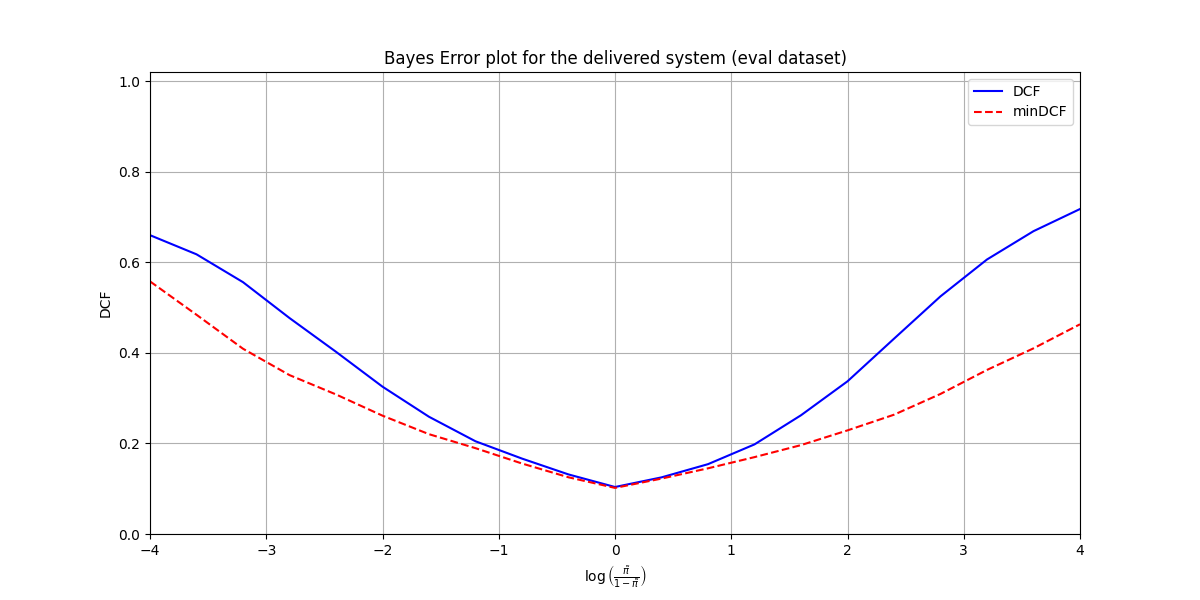
\includegraphics[width=\textwidth]{./plot/eval/delivered.png}
    \end{subfigure}
    \caption{Bayes error plot for the delivered system on the test set.}
    \label{fig:Delivered_System}
\end{figure}
\noindent
We can see that the delivered system is not well calibrated, and the DCF is higher than the minDCF for our target application and for priors at the extremes of the plot.
\nnl
We will now present the results of the single models, as well as the fused ones, on the test set.

\subsection*{Single and Fused Models}
\begin{table}[H]
    \centering
    \begin{tabular}{|l|c|}
        \hline
        \rowcolor{blue!10}
        \textbf{Model} & \textbf{DCF}                     \\
        \hline
        QLR            & 0.494                            \\
        \hline
        RBF SVM        & 0.402                            \\
        \hline
        GMM            & \textcolor{cyan}{\textbf{0.195}} \\
        \hline
        QLR + RBF SVM  & 0.448                            \\
        \hline
        QLR + GMM      & 0.344                            \\
        \hline
        RBF SVM + GMM  & 0.299                            \\
        \hline
        \makecell{QLR + RBF SVM + GMM                     \\ (Delivered System)} & 0.363                            \\
        \hline
    \end{tabular}
    \caption{Model Performance for Application Prior 0.1: DCF}
    \label{tab:model_performance}
\end{table}

\begin{figure}[H]
    \centering
    \begin{subfigure}[t]{0.6\textwidth}
        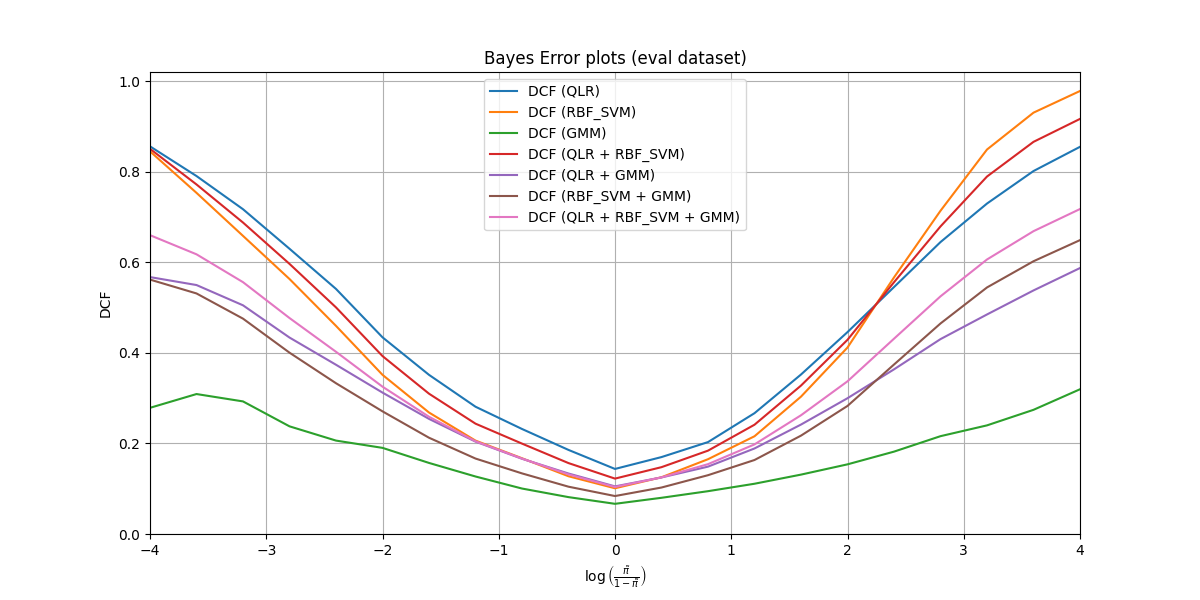
\includegraphics[width=\textwidth]{./plot/eval/DCF_eval.png}
    \end{subfigure}
    \caption{Bayes error plot for the single models and their fusion on the test set.}
    \label{fig:DCF_eval}
\end{figure}
\noindent
We can see that the GMM model is the best model in terms of DCF, with a value of 0.195. Our delivered system was not the best choice possible, and we could have obtained better results by using the GMM model alone.
\nl
After all the fusion of the models was not strictly necessary, and the GMM model was also able to achieve similar results during the training phase.

\subsection*{Calibration of Single Models}
We have seen that the models are not well calibrated, and we will now try to calibrate them using the Prior Weighted Logistic Regression model.
\nl
We will present the results of the calibration step for the single models. We are not going to present the results for the fused models.
\begin{table}[H]
    \centering
    \begin{tabular}{|c|c|c|}
        \hline
        \rowcolor{blue!10}
        \textbf{Model} & \textbf{minDCF} & \textbf{calDCF} \\
        \hline
        QLR            & 0.351           & 0.370           \\
        \hline
        RBF SVM        & 0.262           & 0.288           \\
        \hline
        GMM            & 0.183           & 0.210           \\
        \hline
    \end{tabular}
    \caption{Calibration of the single models on the test set (application prior = 0.1)}
    \label{tab:calibration_single_models}
\end{table}
\noindent
We can see that the calibration step is able to improve the performances of the models, especially for the QLR and SVM models. As in the training phase, the GMM model is already well calibrated and the calibration step seems to worsen the performances of the model.
\nl
Here instead is the bayes error plot for the single models after the calibration step.

\begin{figure}[H]
    \centering
    \begin{subfigure}[t]{0.32\textwidth}
        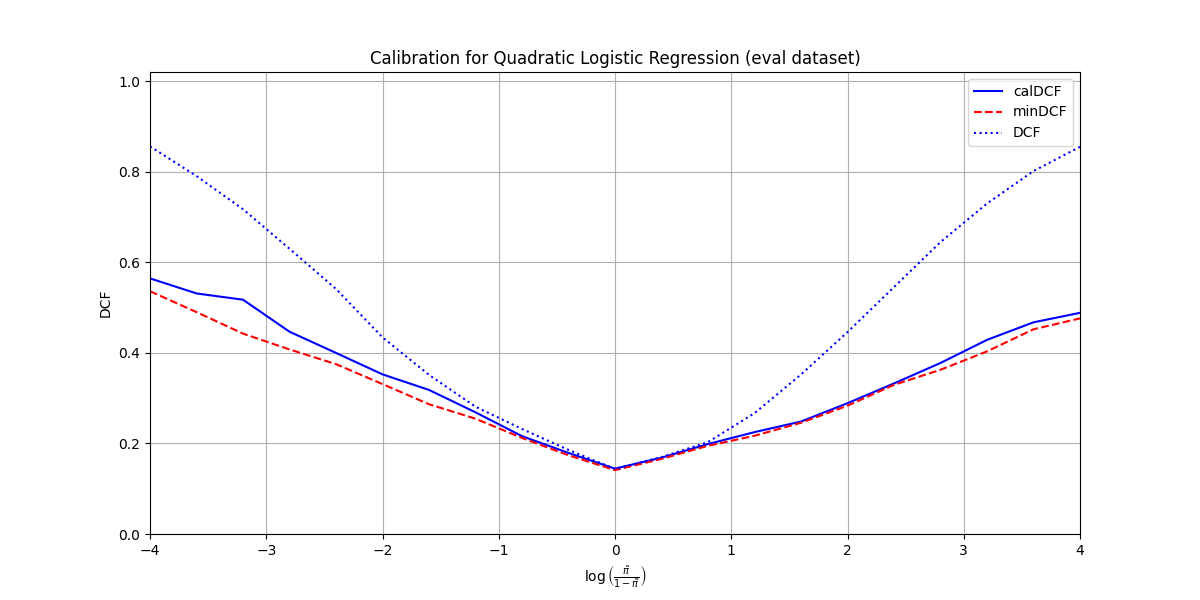
\includegraphics[width=\textwidth]{./plot/eval/eval_calib_QLR.png}
    \end{subfigure}
    \hfill
    \begin{subfigure}[t]{0.32\textwidth}
        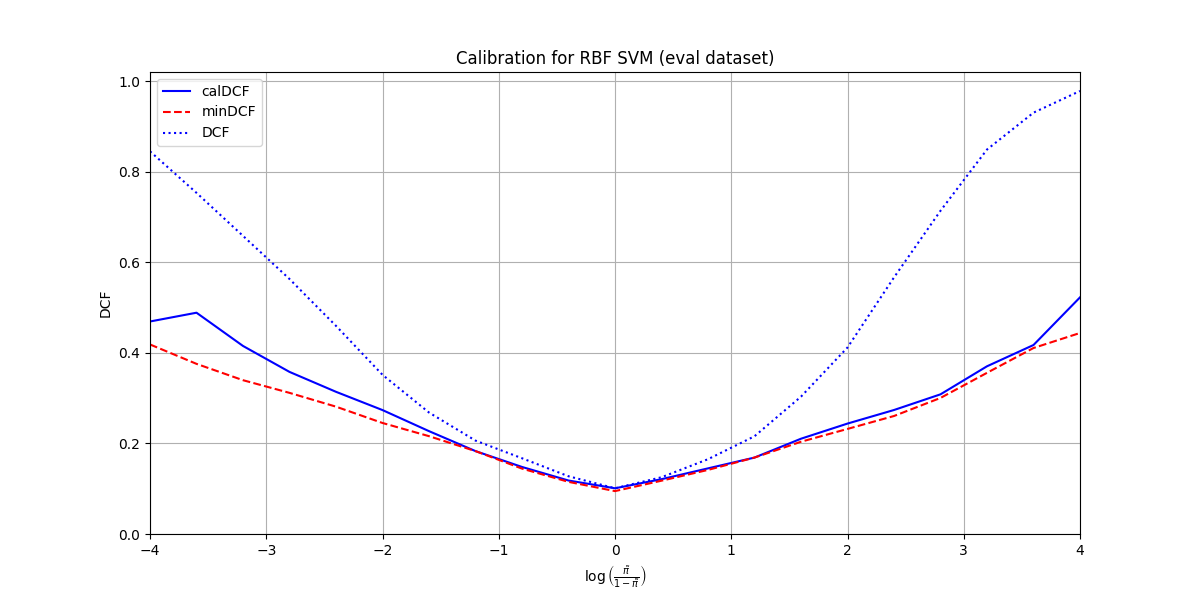
\includegraphics[width=\textwidth]{./plot/eval/eval_calib_RBF_SVM.png}
    \end{subfigure}
    \hfill
    \begin{subfigure}[t]{0.32\textwidth}
        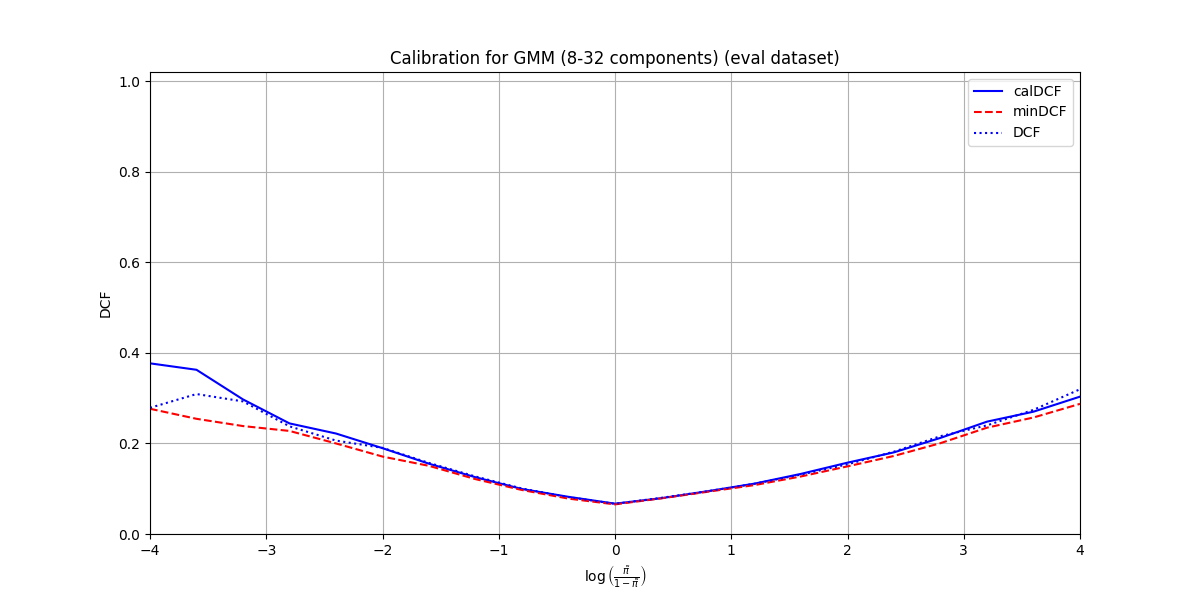
\includegraphics[width=\textwidth]{./plot/eval/eval_calib_GMM.png}
    \end{subfigure}

    \caption{Bayes error plot for the single models after the calibration step on the test set.}
    \label{fig:calibration_single_models}
\end{figure}
\noindent
What we have said for the target application is confirmed also for other priors: calibration greatly improves the performances of the QLR and SVM models, while it worsens the performances of the GMM model.
\nnl
After the calibration step the GMM model is still the best model in terms of DCF, with a value of 0.210. This confirms what we have seen during the training phase.

\subsection*{Analysis of the training strategy}
In this last section we are going to use the test set to analyze the training strategy we have used and see if it was effective in improving the performances of the models.
\nl
We are only going to consider the GMM model, but this analysis could be extended to the other models as well.
\nnl
We will consider the following training strategies:
\begin{itemize}
    \item Train the models using the training part of the original dataset
    \item Repeating the training step for GMM model with full, diagonal and tied covariance matrix, with a different number of components
    \item Use these models to classify the samples in the test set and calculate the resulting DCF and minDCF
\end{itemize}

\begin{figure}[H]
    \centering
    \begin{subfigure}[t]{0.6\textwidth}
        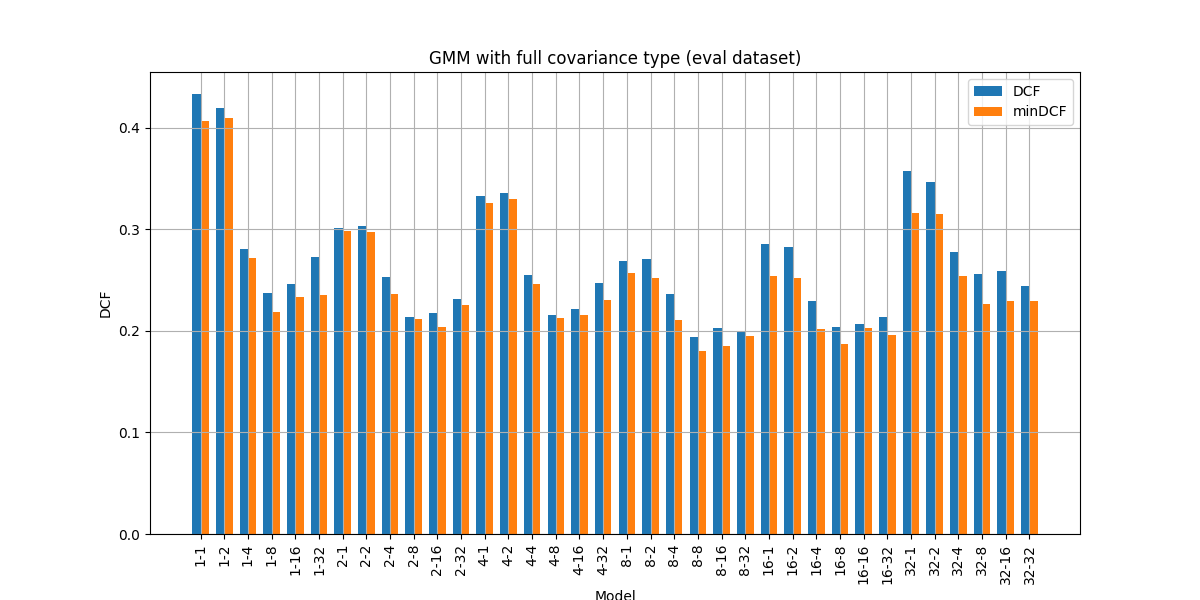
\includegraphics[width=\textwidth]{./plot/eval/GMM/gmm_full.png}
    \end{subfigure}
    \caption{DCF and minDCF for the GMM classifier as a function of the number of components (eval dataset).}
    \label{fig:gmm_full_eval}
\end{figure}

\begin{figure}[H]
    \centering
    \begin{subfigure}[t]{0.6\textwidth}
        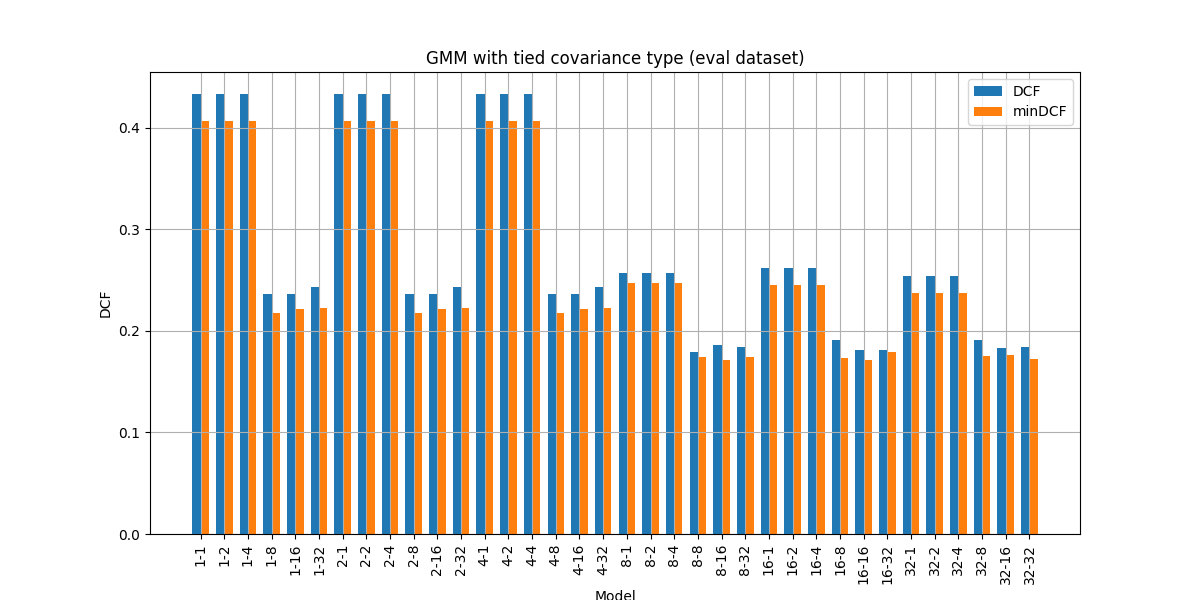
\includegraphics[width=\textwidth]{./plot/eval/GMM/gmm_tied.png}
    \end{subfigure}
    \caption{DCF and minDCF for the GMM (tied covariance matrix) classifier as a function of the number of components (eval dataset).}
    \label{fig:gmm_tied_eval}
\end{figure}

\begin{figure}[H]
    \centering
    \begin{subfigure}[t]{0.6\textwidth}
        \includegraphics[width=\textwidth]{./plot/eval/GMM/gmm_diag.png}
    \end{subfigure}
    \caption{DCF and minDCF for the GMM (diagonal covariance matrix) classifier as a function of the number of components (eval dataset).}
    \label{fig:gmm_diag_eval}
\end{figure}

As we can see from the figures, the best results are obtained with the GMM model with diagonal covariance offers good performances, but we have to mention that the tied covariance matrix model performs surprisingly well compared to the training phase.
\nl
To conclude we can say that the training strategy we have used for the GMM model was effective in improving the performances.

\chapter{Conclusions}
In this project we have analyzed the performances of different models on a dataset of speech features. We have trained different models (Quadratic Logistic Regression, SVM with RBF kernel, Gaussian Mixture Model) and we have compared them in terms of DCF and minDCF.
\nnl
The model we decided to deliver turned out not to be the best option, and we could have obtained better results by using the GMM model alone.
\nl
For what concerns the training strategy for this model we can say that it was effective in improving the performances of the model.

\end{document}